\chapter{Gas Electron Multiplier} % (fold)
\label{cha:gas_electron_multiplier}
\begin{chapquote}
{Freeman Dyson}
``New directions in science are launched by new tools much more often than by new concepts.''
\end{chapquote}
\todo[inline]{Add HV divider and circuit readout board}
\todo[inline]{Why we need test beam studies}
\todo[inline]{Add GE1/1 long and short detector description.}

In this chapter, the GEM detector technology is introduced which are proposed for the CMS muons system upgrade during the long shutdown-2 period. 
The properties of these GEM detectors were scrutinized during different beam test campaigns carried out at the CERN SPS beam test facility.
The first half of this chapter deals with the measurements performed on prototypes of CMS GEM detectors using the data collected during  different beam tests. 
The characterisation of GEM foils developed in India for the CMS upgrade is described in the last part of the chapter.

\section{Introduction} % (fold)
\label{sec:introduction}
The invention of Multi-Wire Proportional Chamber (MWPC) in 1968 by Georges Charpak was one of the major breakthroughs in the development of gaseous detectors since it had better rate capability vis-a-vis its predecessors~\cite{Charpak1968}. 
This invention also leads to a Nobel prize for George Charpak in 1992. 
The design and performance of MWPC have improved progressively through all these years.
However, because of our increasing demands with the acquired knowledge about particle detection, it has reached its limitation in terms of the maximum rate capability and detector granularity.
In 1988, Anton Oed invented the Micro-Strip Gas Counter (MSGC) which had a position resolution of few tens of microns and could overcome the rate limitation arising due to positive-ion accumulation in the gas volume. 
Also, it could sustain a particle flux greater than few $MHz/mm^2$. Although, these kind of detectors were very impressive but the long-term study revealed the following shortcomings:
\begin{enumerate}
	\item Accumulation of the ions on the electrodes, which affects the gain and age of the detector.
	\item In some cases, the passage of highly ionising particles could lead to a destructive discharge in the detector medium.
\end{enumerate}
These drawbacks of the MSGC lead to the development of Micro-Pattern Gaseous Detectors (MPGD).
This class of detectors, specifically the Gas Electron Multiplier (GEM)~\cite{Sauli1997,Sauli1999,detector:1732870}, could provide an unprecedented spatial resolution, larger sensitive/detection area, with higher rate capability and good operational stability over the longer operating periods.
Several new studies also revealed that under certain circumstances these detectors might be less vulnerable to the radiation-induced ageing than the standard silicon microstrip detectors~\cite{TITOV2004,Titov2002}.

Because of their efficient detection qualities and high rate capabilities, GEM detectors have been already used in various experiments like COMPASS, TOTEM, LHCb. Recently, it was proposed for the CMS muon detector system upgrade. A brief description of the working and properties of GEM detectors is provided in the following sections.
% section introduction (end)

\section{Design and working principle of GEM detector} % (fold)
\label{sec:design_and_working_principle_of_gem}

GEM is a relatively new concept introduced by Fabio Sauli~\cite{Sauli1997} at CERN, which consists of a thin polyimide sheet (usually a thin Kapton foil~\cite{Kapton-sheet} with thickness 50 $\mu m$) coated with metal on its both sides. It is chemically pierced to a regular array of holes using the photolithography and acid etching processes~\cite{Benlloch1998}, as shown in Fig.~\ref{fig:gem} (left).
\begin{figure}[!htbp]
    \centering
    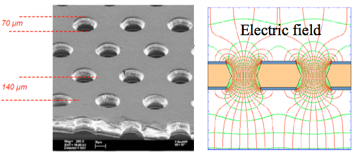
\includegraphics[width=0.95\textwidth]{figures/GEM/KEKDTP3.jpg}
    \caption{A cross-sectional view of a GEM foil etched with holes (left). The strong electric field generated in the vicinity and inside of the holes on the application of the potential across the foil (right).}
    \label{fig:gem}
\end{figure}

A potential difference is applied between the two copper layers which create a high electric field inside the holes (Fig.~\ref{fig:gem}) and is given as
\begin{equation}
    E = \frac{V}{d}
\end{equation}
where E is the electric field inside a hole in the GEM foil, V is the voltage applied between the two copper layers and d is the thickness of the GEM foil.
% Since the Kapton\footnote{Kapton was chosen as the insulating layer as it has very good insulating power along with that it can sustain very high radiation along with that it works with wide range of temperature. It is a plastic polyamide created by DuPont.} foil is very thin, around 50 $\mu m$, so a high electric field density will be created in the hole which is shown in Fig.~\ref{fig:gem} (right).
\begin{figure}[htbp]
    \centering
    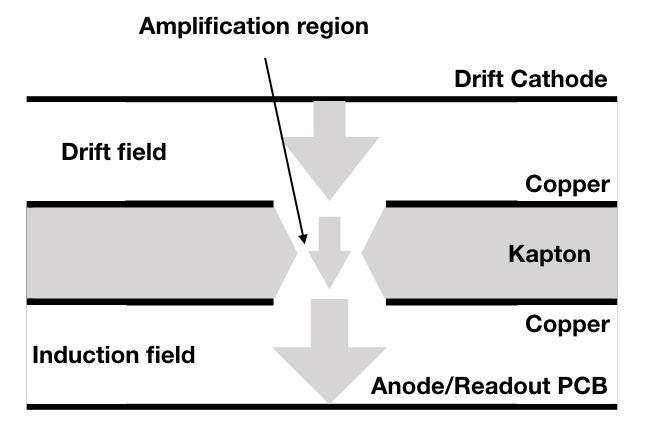
\includegraphics[width=0.55\textwidth]{figures/GEM/SingleGEM_Detector.jpeg}
    \caption{Outline of a single GEM detector.}
    \label{fig:gemOutline}
\end{figure}

To illustrate the working of a GEM detector, the active detector medium could be divided into three different regions: drift, amplification and induction regions, as shown in Fig.~\ref{fig:gemOutline}.
The passage of a charged particle leads to ionization in the drift region, and the generated primary electrons drift towards the amplification region (i.e., through GEM holes). 
The electrons gain kinetic energy from the intense electric field inside the holes sufficient to produce secondary ionizations, eventually, leading to an avalanche multiplication.
Finally, in the induction region, all the electrons from the amplification region are collected on the readout plane. 

To avoid the problem of electrical breakdown, several GEM foils operating at lower voltages, are stacked together in between the drift cathode and the readout board.
For such detector configurations, the through transfer region takes most of the almost all the electrons from one GEM foil to another.
In view of the fact that the total gain of a detector is given as the product of the individual gain of each foil, gains up to an order of $10^5$ can be achieved in this way.
In this configuration, the detector can reach its maximum gain without any or with the least probability of electric discharge.

% Also, the total gain is the product of the individual gain of each foil, so the gain up to $10^5$ can be achieved in this way.
% In this configuration, it can reach maximum gain without any discharge or least probable.
% In Fig.~\ref{fig:tripleGEM_discharge_gain}, 
The gain and discharge probability are compared for the single, double and triple-layered GEM detectors are shown in Fig.~\ref{fig:tripleGEM_discharge_gain}, which clearly indicates that the triple GEM detectors can achieve a gain beyond $10^4$ without any electrical discharge.
Also, the signal readout by the electrode is pretty fast as it uses only electrons to read the signal. 
Multi-layered boards could be used to achieve a two-dimensional readout from these detectors.
\begin{figure}[!htbp]
    \centering
    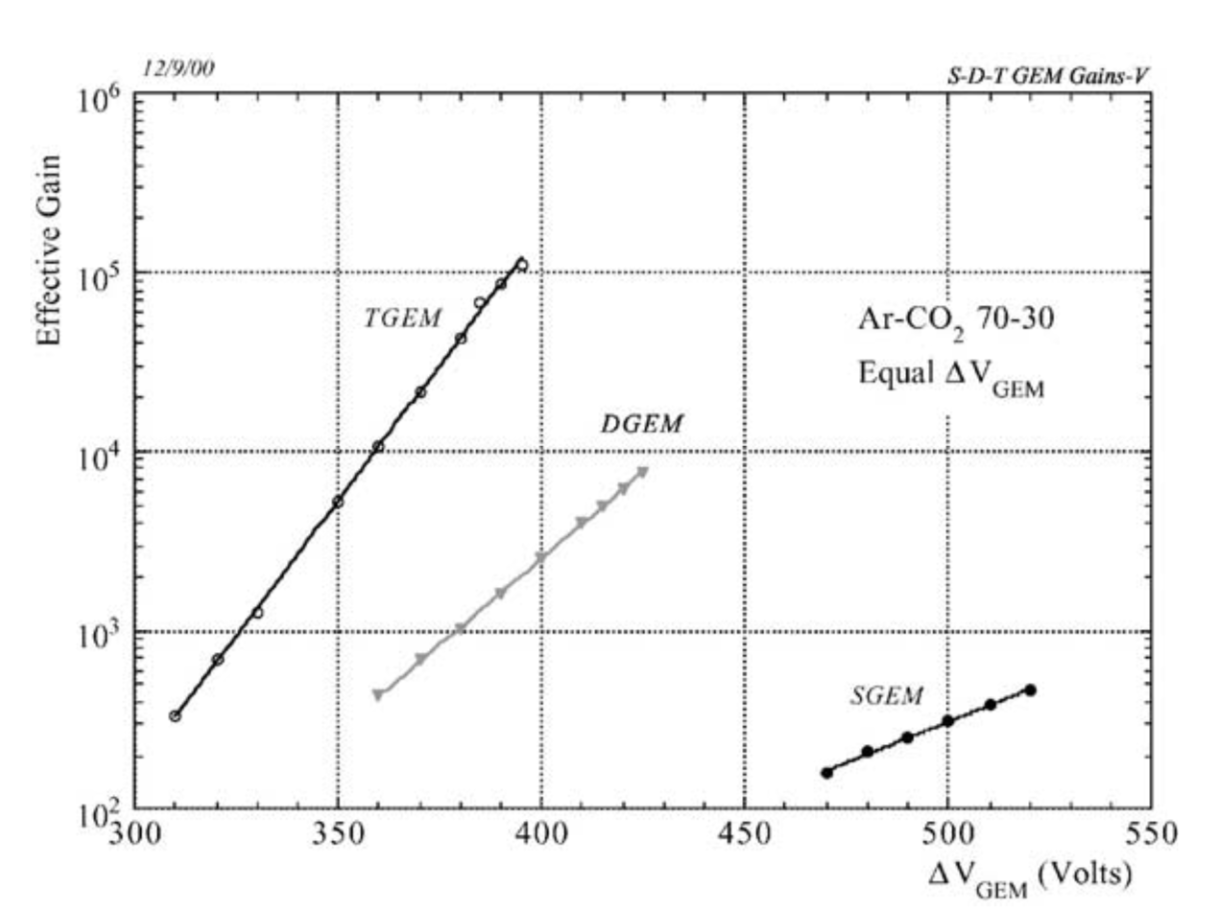
\includegraphics[width=0.5\textwidth]{figures/GEM/Comp_threeGEMS_Gain.png}%
    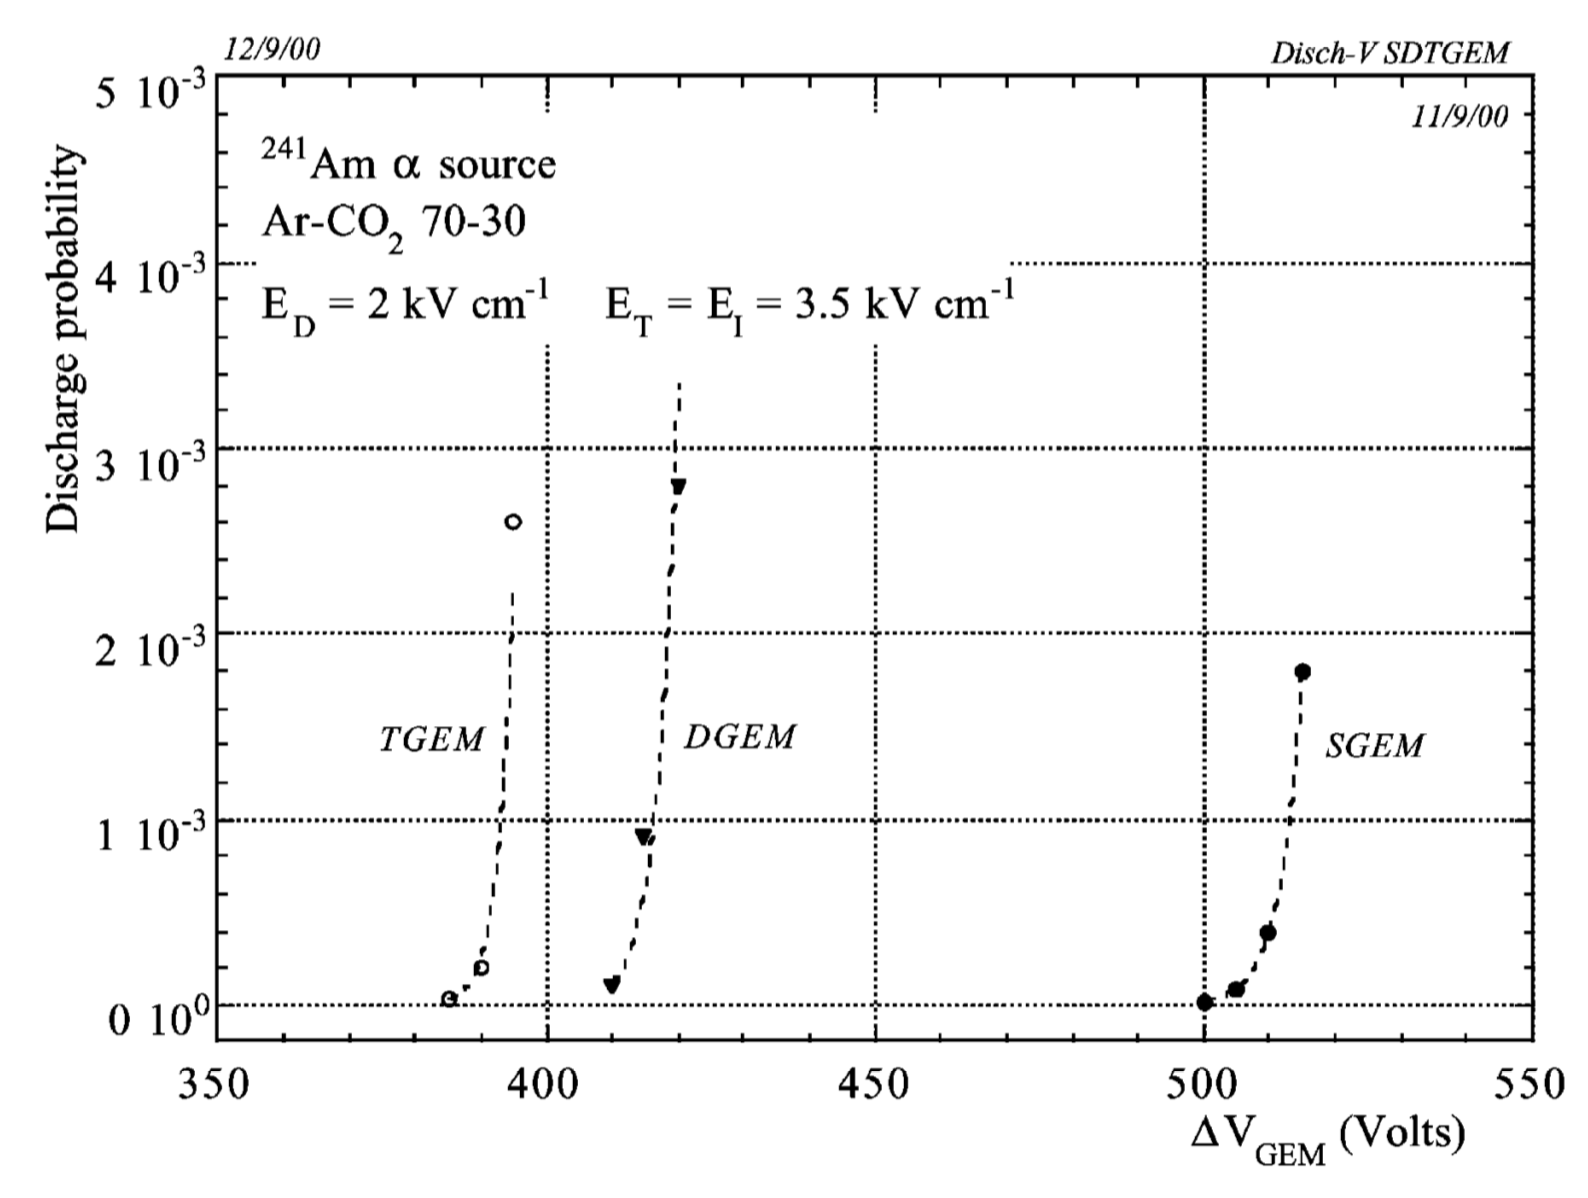
\includegraphics[width=0.5\textwidth]{figures/GEM/Comp_threeGEMS_DischargeProbability.png}
    \caption{Comparison of total effective gain on anode as a function of applied voltage for single, double and triple layred GEM detectors (left). The discharge probality as a function of applied voltage is shown for the single, double and triple layred GEM detectors (right)~\cite{Bachmann2002}.}
    \label{fig:tripleGEM_discharge_gain}
\end{figure}

A detector arrangement where three GEM foils are stacked together is known as a ``\textit{\textbf{Triple-GEM detector}}'', as shown in Fig.~\ref{fig:gemgaps}. Such a detector configuration is proposed for the CMS Phase-II upgrade and is discussed in the following section.
\begin{figure}[!htbp]
    \begin{center}
        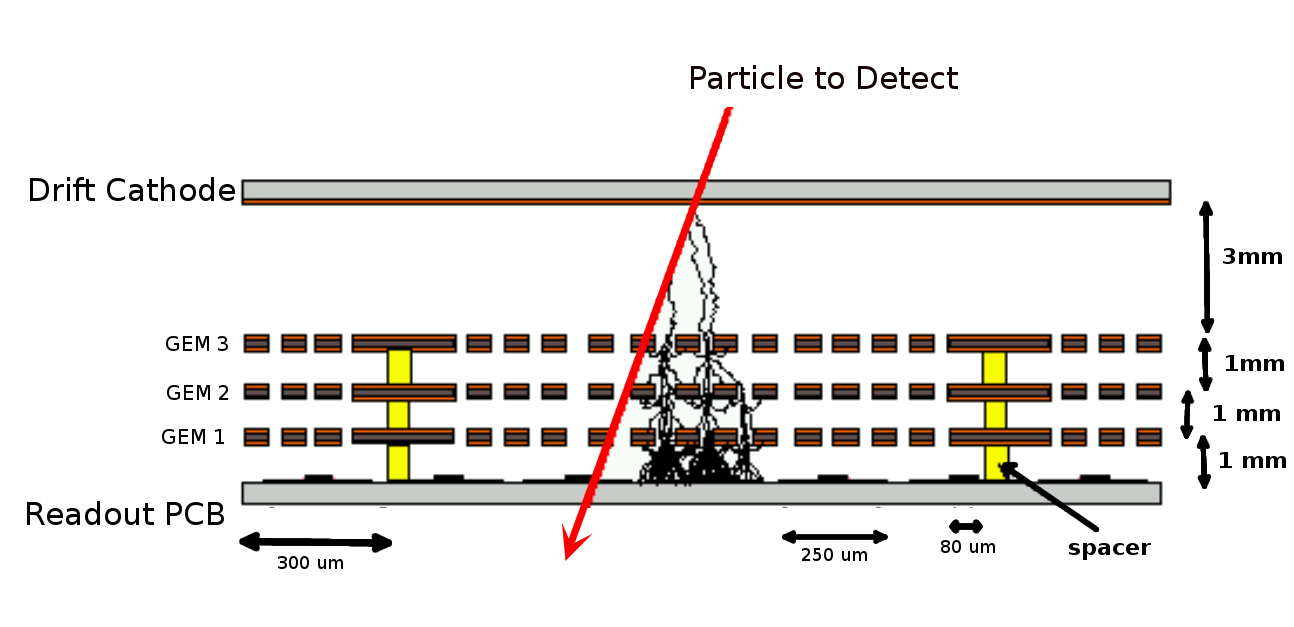
\includegraphics[width=0.85\textwidth]{figures/GEM/triple_gem.png}
        \caption{The working mechanism of a GEM detector.}
        \label{fig:gemgaps}
    \end{center}
\end{figure} 
% section design_and_working_principle_of_gem (end)


\section{GEM for the CMS Phase-II Upgrade} % (fold)
\label{sec:gem_for_cms}
As pointed out in Sec.~\ref{sub:the_muon_system},  the CMS Collaboration has finalised to install GEM detectors in the pseudo-rapidity region $1.6 < |\eta| < 2.2$.
These detectors will support the existing CSC muon sub-system to improve the muon triggering and tracking capabilities in the forward region~\cite{Colaleo:2021453}.
The combined operation of CSC and GEM detectors will lead to a precise measurement of the muon bending angle at the trigger level, thus strongly reducing the rate of muon mis-reconstruction.

This CMS muon detector system upgrade is carried out to achieve the following goals:
\begin{itemize}
    \item Re-establish the redundancy in the forward region beyond $\eta = 1.6$
    \item Improve the muon tracking performance during the high-luminosity LHC operation.
    % \item The combined operation of CSC and GEM detectors allows a measurement of the bending angle at the trigger level, thus strongly reducing the rate of mis-measured muons driving the triggers rate.
\end{itemize}
% \subsection{GE1/1 Details}
The installation of GEM detectors is proposed during the period of Long Shutdown-2 (2019-2020).
The upgrade project is named as CMS GE1/1 upgrade, where the letter ``G'' stands for GEM, ``E'' stands for End-cap, the first ``1'' corresponds to the first muon station and the second ``1'' corresponds to the first ring of the station.
Analogously, the GEM detectors to be installed in the CMS detector are referred to as GE1/1 detectors.
The detectors will be inserted in front of the ME1/1 station and into the slots originally foreseen for the RPC detectors, as shown in Fig.~\ref{fig:GE1/1pos}. 
\begin{figure}[!htbp]
    \centering
    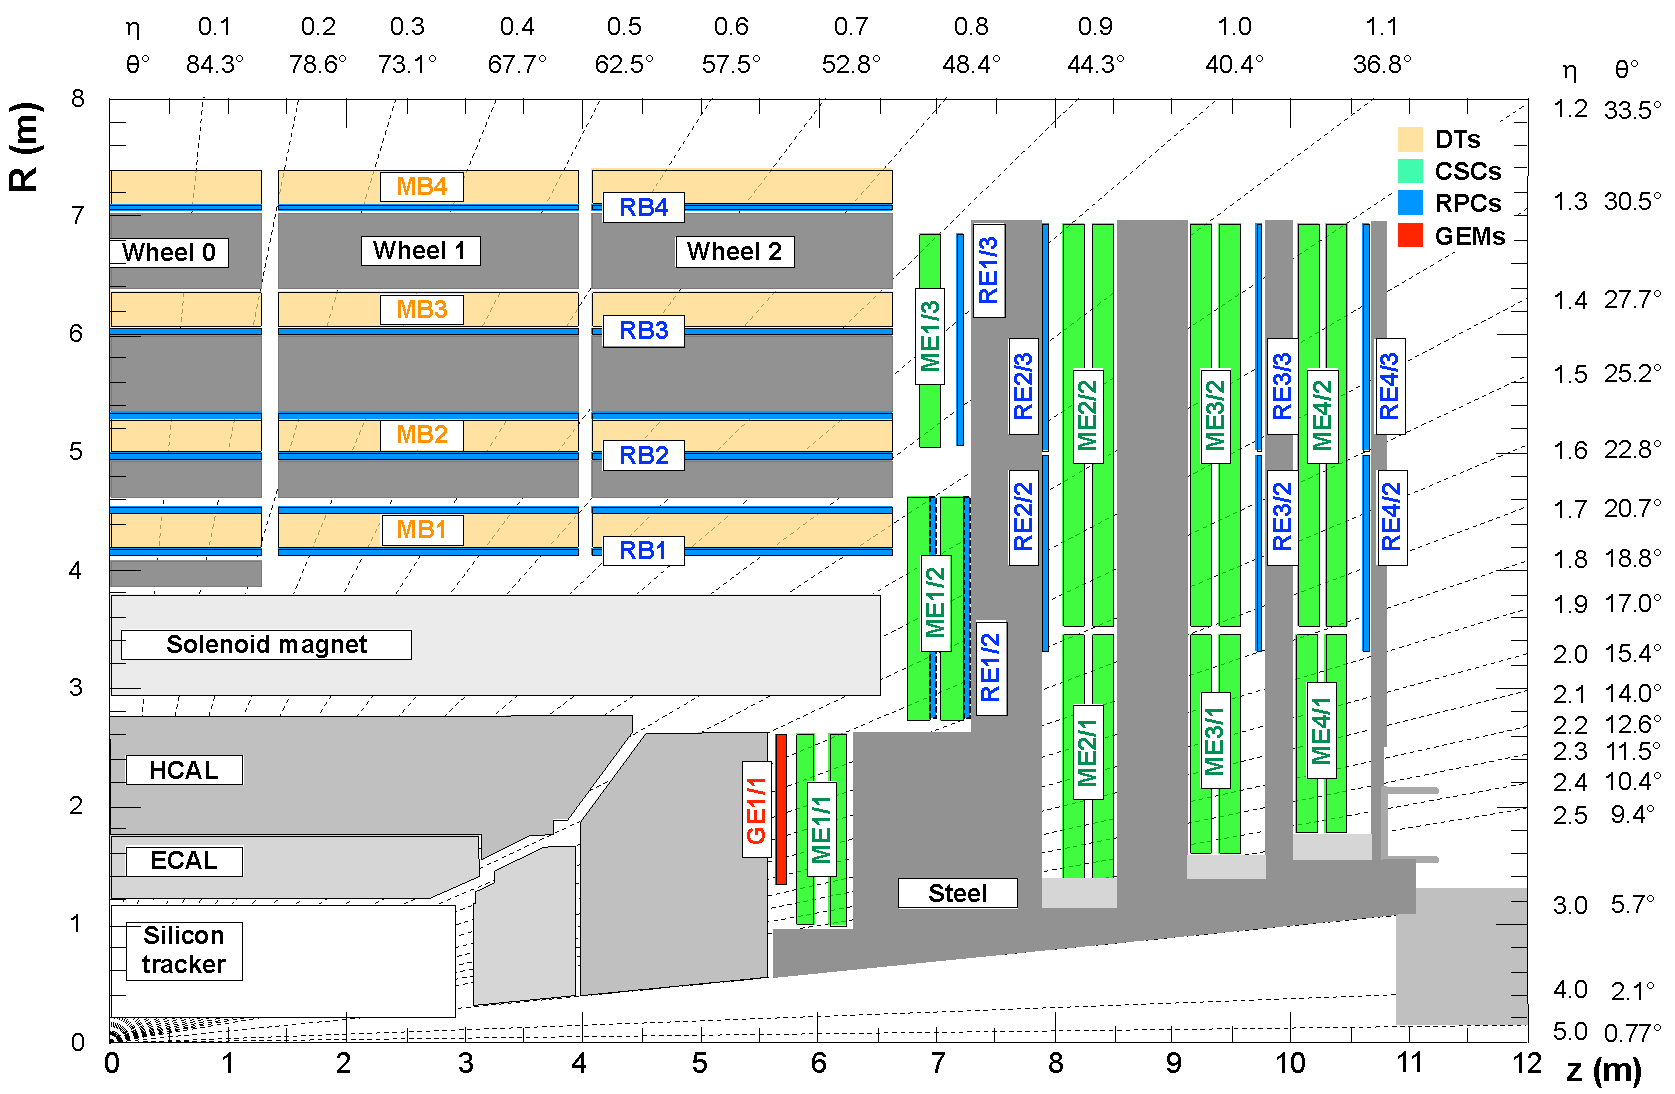
\includegraphics[width=0.95\textwidth]{figures/GEM/cms_upg_o_g_b_ni_ge1_r_140227.pdf}
    \caption{A cross-sectional view of the CMS quadrant highlighting the location of GEM detectors (red).}
    \label{fig:GE1/1pos}
\end{figure}

\subsection{CMS GE1/1 Detector Specification} % (fold)
\label{sub:GE1/1_detector_details}
A typical GE1/1 detector is trapezoidal in shape with an active area of $990~\times~(220-445)~mm^2$.
The shape and size of the detector was decided based on the geometry of vacant high-$\eta$ region in the CMS muon endcap regions.
A GE1/1 chamber consists of a Triple-GEM detector having a $3/1/2/1~mm$ (drift/transfer 1/transfer 2/induction) electrode gap configuration, as shown in Fig. \ref{fig:tripple-gem}.
\begin{figure}[!htbp]
    \begin{center}
        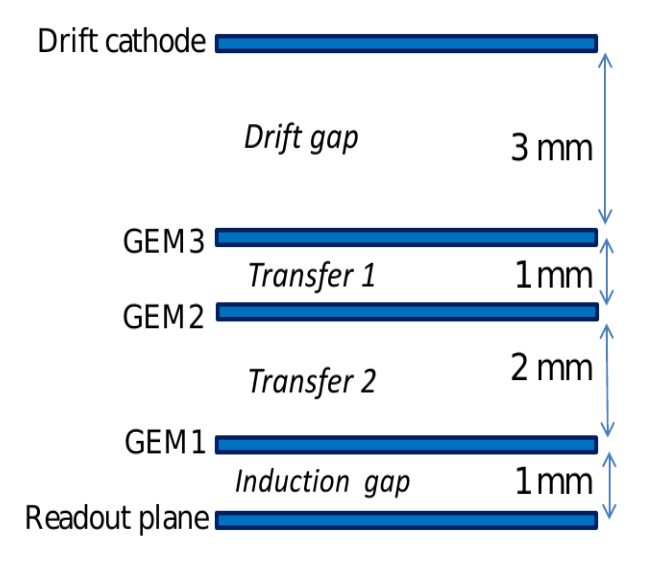
\includegraphics[width=0.45\textwidth]{figures/GEM/tripple-gem.png}
        \caption{The layout of different GEM layers inside a CMS GE1/1 detector.}
        \label{fig:tripple-gem}
    \end{center}
\end{figure} 
% ($50~\mu m$ thick Kapton foil with $5\mu m$ copper on both sides) 
The GEM foil consists of a thin Kapton foil ($50~\mu m$ thick) with a copper clad ($5~\mu m$) on both sides.
The detector readout board is divided into eight $\eta$-partitions with 384 strips.
Each strip is radially oriented along the long side of the detector with a pitch varying from $0.6~mm$ (short side) to $1.2~mm$ (long side).
Each partition is subdivided along the $\phi$-coordinate into three readout sectors with 128 strips or channels per sector. The $\eta$ partition and $\phi$ portions of the GEM detector are shown in Fig.~\ref{fig:gemTrapezoidal}.
\begin{figure}[!htbp]
    \begin{center}
        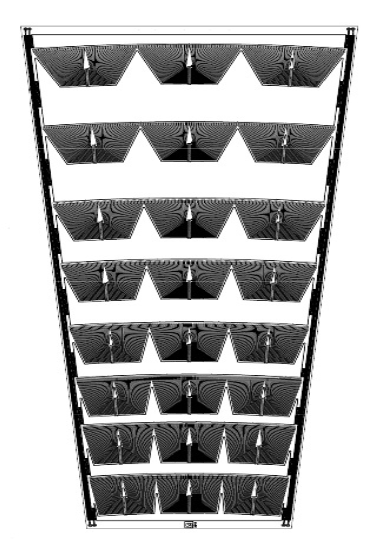
\includegraphics[angle=-90,width=0.75\textwidth]{figures/GEM/gemTrapezoidal.png}
        \caption{Drawing of a large trapezoidal CMS GEM chamber showing $8-\eta$ and $3-\phi$ par partitions.}
        \label{fig:gemTrapezoidal}
    \end{center}
\end{figure} 
To improve tracking capabilities, two GEM chambers will be mounted face-to-face to form a double layer called ``\textit{Super-Chamber}".
Thus each Super-Chamber will provide two impact points for each muon track.
The full layer by layer mechanical design of a GEM chamber is shown in Fig.~\ref{fig:GE1/1}. 
The main parts in a GEM detector are GEM foil, drift plane, readout board, shielding, high voltage divider, etc.
\begin{figure}[!htbp]
    \begin{center}
        \includegraphics[width=0.95\textwidth]{figures/GEM/GE11cad.png}
        \caption{Layer by layer view of GEM detector}
        \label{fig:GE1/1}
    \end{center}
\end{figure} 
\todo[inline]{Add a para on fig~\ref{fig:GE1/1}}
\todo[inline]{Add a para on GE1/1 fabrication}
% \begin{figure}[!htbp]
% \centering
% 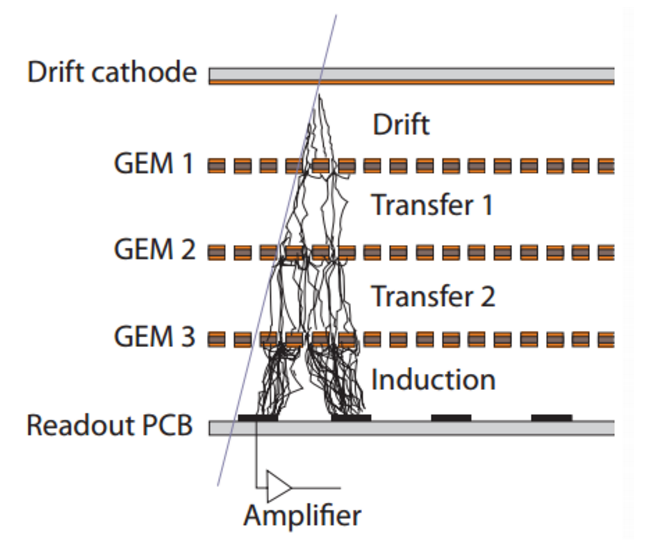
\includegraphics[width=2.0in]{figures/GEM/GEMCascade.png}
% \caption{Generic triple-GEM chamber, showing drift, transfer, and signal induction gap regions within the detector.}
% \label{GEM:cascade}
% \end{figure}

\subsection{GE1/1 Beam Test Studies}
The GE1/1 detector was tested using 150 GeV muon and pion beams at CERN SPS beam test facility during October-December 2014. 

The goal of the beam test campaign was to measure the efficiency, space \& time resolution, and the cluster size of the CMS GEM detector. 
The detectors that were tested includes GE11\_IV and GE11\_IV\_GIF detectors.
% (detectors naming convention and its details are mentioned in the appendix~\ref{cha:GE1/1_detector_generations}).
Both GE11\_IV and GE1/1\_IV\_GIF are generation\footnote{The different generations of GE1/1 are described in appendix~\ref{cha:ge11_detector_generations}} IV GE1/1 detectors but GE1/1\_IV\_GIF was irradiated with the gamma-ray at the CERN gamma-ray irradiation facility\footnote{The GIF bunker contains a $^{137}Cs$ source of 566 GBq. This emits gamma rays of 662 keV. The detector was placed 30 cm from the source where the particle rate was of the order of 100 $kHz/cm^2$. This allowed accumulating the charge in twelve month which will be equivalent to the 10-year operation of GEM detector in LHC environment~\cite{Merlin2013}.} for 1 year to perform ageing studies~\cite{Merlin2013}. Also, several important parameters like electric field, voltage across each GEM foil and the rate and gain were measured and shown in appendix~\ref{cha:ge1_1_measured_parameters}.

% This is also a generation IV GE11 detector. But, for the ageing test this detector was placed at the Gamma Irradiation Facility (GIF) for twelve months.
Two beam test campaign was carried out during October-December 2014.
These campaign held in H2 and H4 beam test area of CERN SPS.
The H2 beam test was held from $6^{th}$ October 2014 to $27^{th}$ October 2014 while the H4 beam test was held from 26 November to 14 December 2014.
The main goal of the H2 beam test was to test the two detectors mentioned above with an $Ar:CO_2$ gas mixture while in H4 beam test the same detector was tested with $Ar:CO_2:CF_4$ gas mixture.
Initially, the plan was to scan each sector of the GEM detectors but due to timing constraints we were just able to scan sector $(i\eta, i\phi)=\{(5,2)\}$ and $(i\eta,i\phi)=\{(1,2),(5,2),(8,2)\}$ during H2 and H4 beam test respectively.  

The data collected during these beam test campaigns were grouped into different run names, based on the electronic setup and gas mixtures used during the data taking. Out of these four set of run ranges were marked as ``\textit{good}'', based on certain data quality checks, for further analysis. These run ranges along with their specification are listed in Table~\ref{tab:gemTBgoldenruns}.

\begin{table}
\begin{tabular}[!htbp]{l l}
\hline
\textbf{Run Name}   &   \textbf{Details}\\
\hline
2014H2C     & Run range: 306-407    \\
            & Threshold for each VFAT strip = 15 VFAT units\footnote{1 VFAT unit = 0.08 fC} = 1.2fC\\
            & Asynchronous mode with respect to the LHC clock \\
            & sector scanned $(i\eta, i\phi)=(5,2)$\\
            & Gas mixture used: $Ar:CO_{2}$=(70:30)\\
\hline
2014H4A     & Run range: 1592-1646 \\
            & Threshold for each VFAT strip = 15 VFAT units = 1.2fC\\
            & Asynchronous mode with respect to the LHC clock \\
            & sector scanned $(i\eta, i\phi)=(5,2)$\\
            & Gas mixture used: $Ar:CO_{2}:CF_4$=(40:15:45)\\
\hline
2014H4C     & Run range: 1868-1906 \\
            & Threshold for each VFAT strip = 15 VFAT units = 1.2fC\\
            & Asynchronous mode with respect to the LHC clock \\
            & sector scanned $(i\eta, i\phi)=(8,2)$\\
            & Gas mixture used: $Ar:CO_{2}:CF_4$=(40:15:45)\\
\hline
2014H4D     & Run range: 2065-2123 \\
            & Threshold for each VFAT strip = 15 VFAT units = 1.2fC\\
            & Asynchronous mode with respect to the LHC clock \\
            & sector scanned $(i\eta, i\phi)=(1,2)$\\             
            & Gas mixture used: $Ar:CO_{2}:CF_4$=(40:15:45)\\
\hline
\end{tabular}
\caption{List of golden runs used to measure the GE1/1 properties.}
\label{tab:gemTBgoldenruns}
\end{table}
% subsection GE1/1_detector_details (end)

\subsubsection{Readout Electronics} % (fold)
\label{ssub:readout_electronics}
Front-end electronics used in the beam test was \textbf{\textit{VFAT2}} chips~\cite{Aspell2007,Berardi2004}.
The upgraded version of the same chip, known as VFAT3, will be used with GE1/1 detectors for Level-1 muon triggering~\cite{Licciulli2017}. Its block diagram is shown in Fig.~\ref{fig:VFAT2block}.

VFAT is a front-end Application Specific Integrated Circuit (ASIC) chip was primarily designed for the readout of sensors in the TOTEM experiment at CERN. 
VFAT chip is used for both triggering and tracking purpose.
For triggering it uses the programmable ``\textit{fast OR}'' information based on a hit in the detector.
It provides a monostable output for the programmed number of channels in a single clock cycle. 
This is called an ``\textit{S-Bit}''. While, for tracking it provides the spatial information strip-wise for every triggered event.

VFAT2 has 128 analog input channels, very low noise pre-amplifier, shaper and comparator attached to it. 
Signal discrimination is done based on the programmable threshold setting and then stored within SRAM\footnote{Static random-access memory (static RAM or SRAM) is a type of semiconductor memory that uses bistable latching circuitry (flip-flop) to store each bit. SRAM exhibits data remanence but it is still volatile in the conventional sense that data is eventually lost when the memory is not powered.} until the trigger information is received. 
It can apply positive as well as negative threshold value to each channel independently. 
This feature is named as ``\textit{TrimDAC}'' and it has two programmable voltages $V_{T1}$ and $V_{T2}$ and the threshold is defined as the difference between these two programmable voltages, i.e., $V_{TH} = V_{T2} - V_{T1}$.

This VFAT chip also provides the facility to mask individual noisy channel.

To synchronize the output of the comparator the monostable block provides 1 clock pulse for each threshold-crossing signal.

\begin{figure}[htbp]
    \centering
    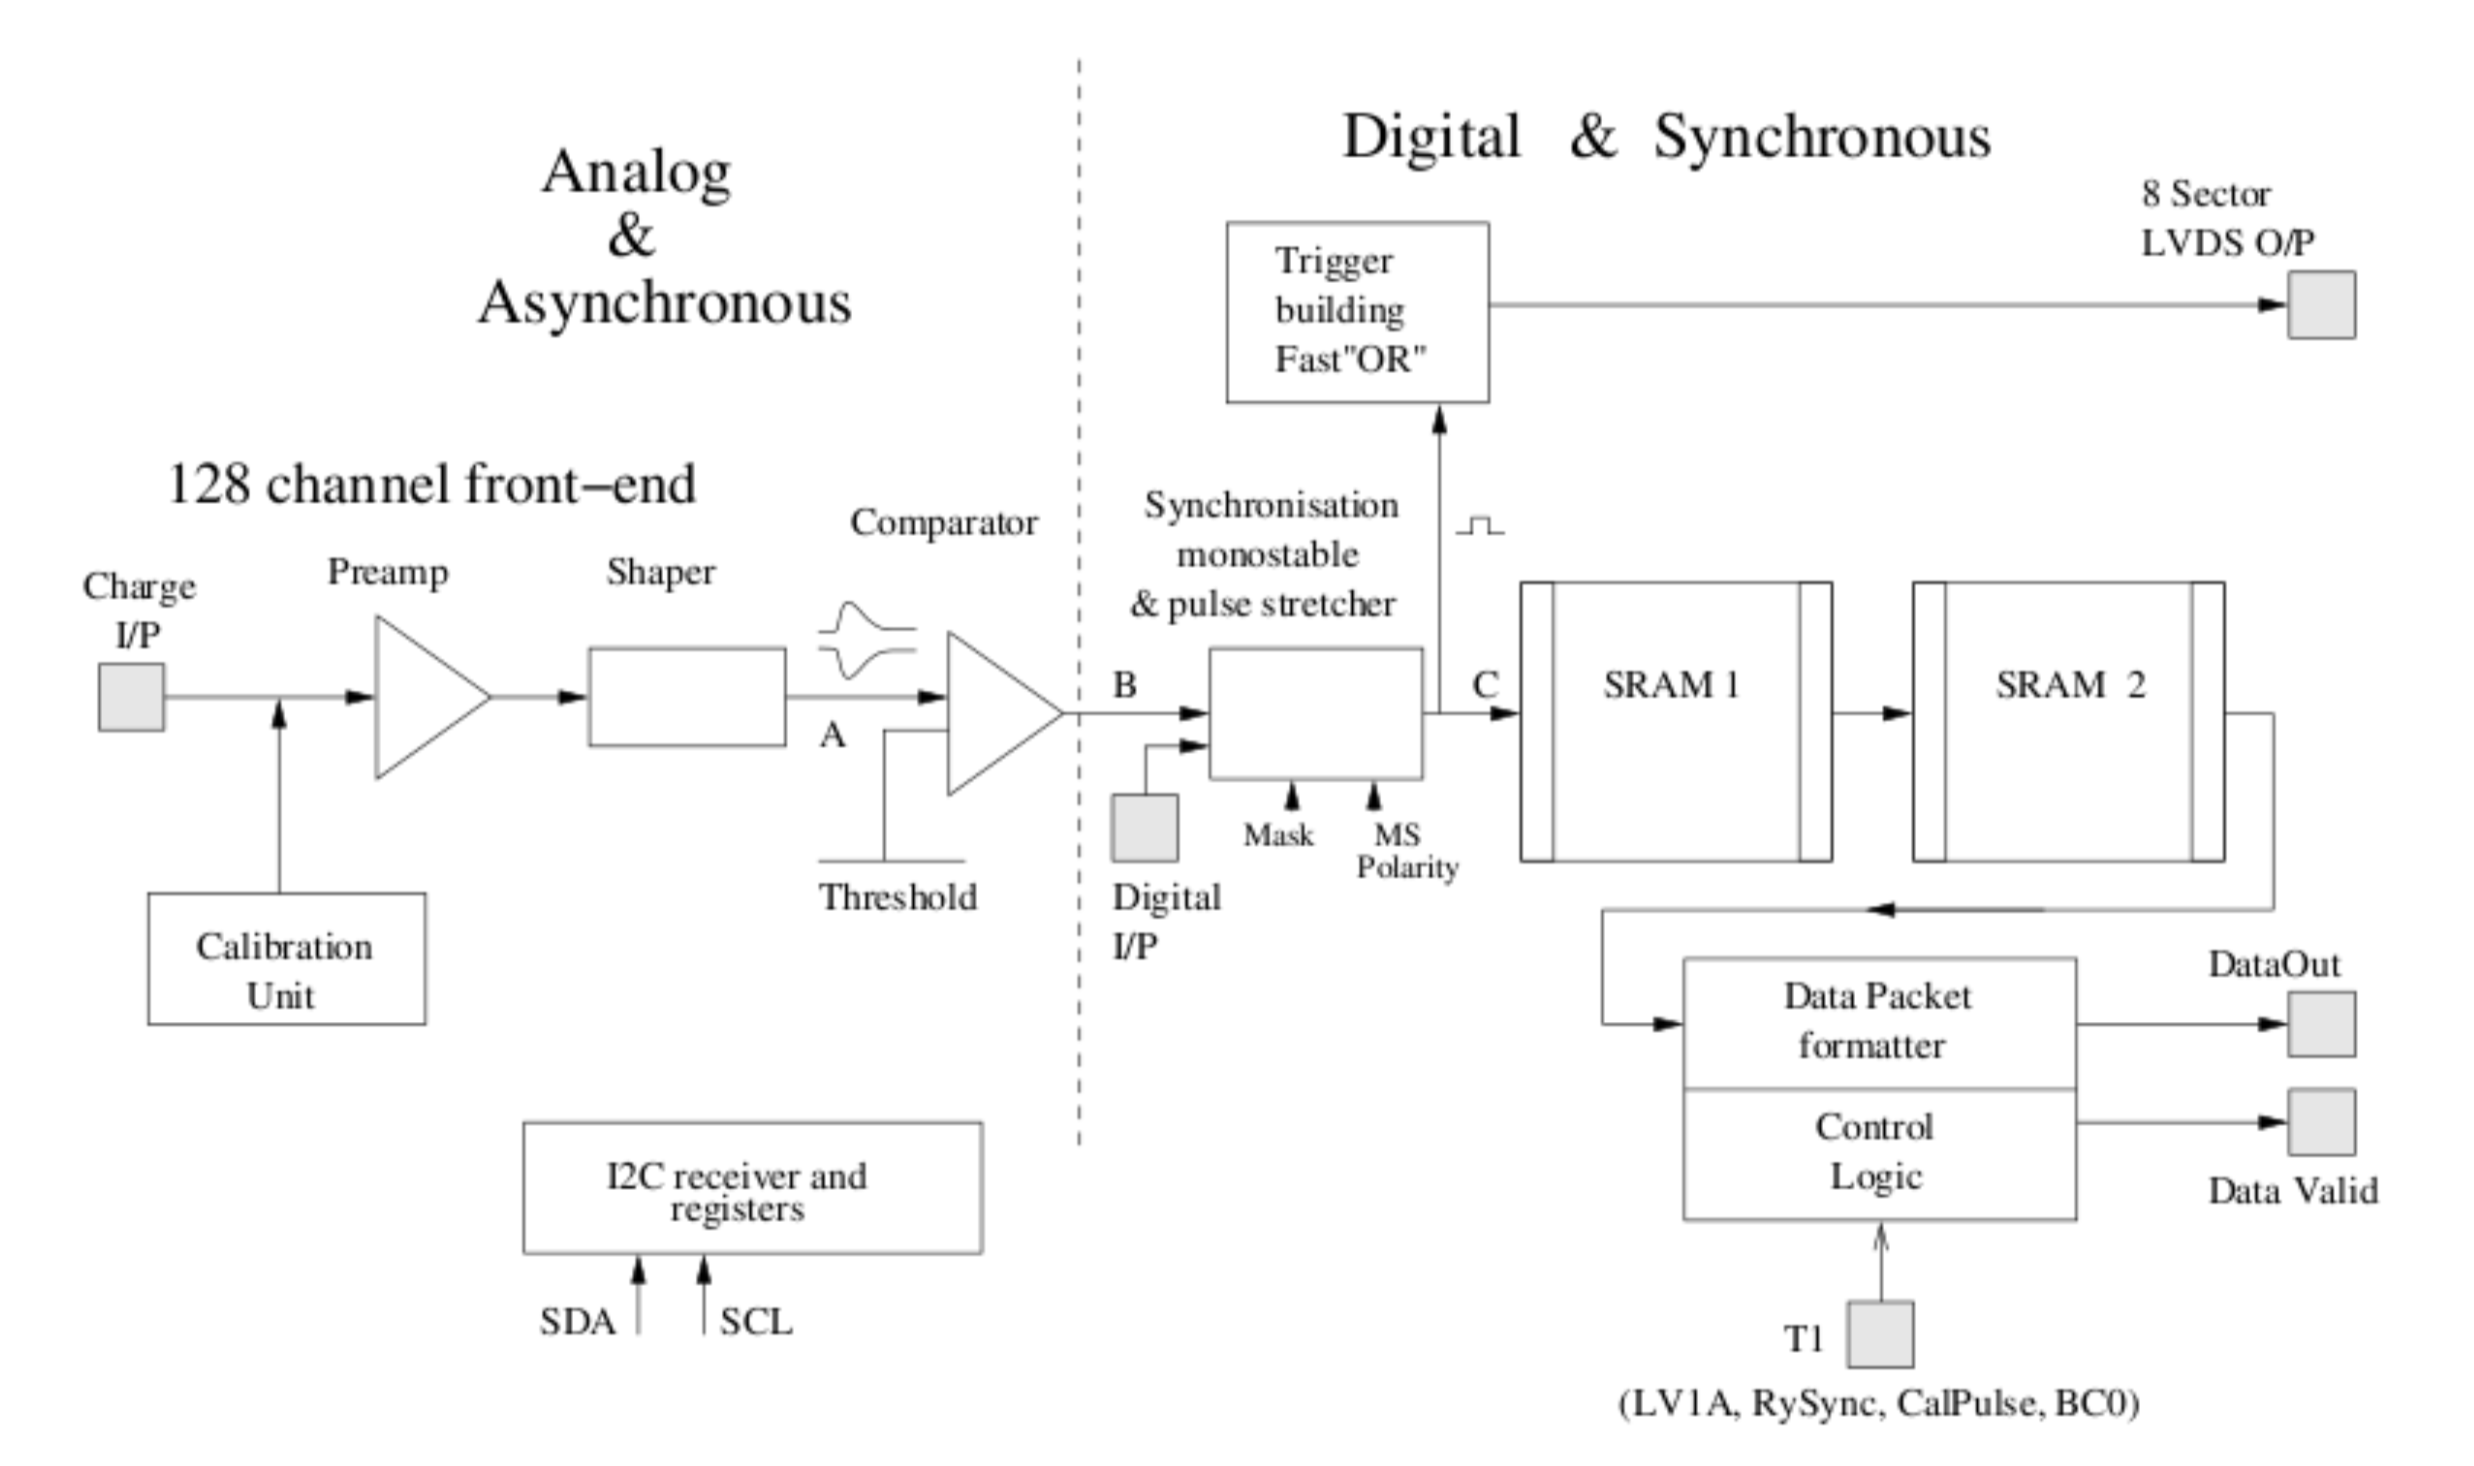
\includegraphics[width=0.95\textwidth]{figures/GEM/VFAT2_chip_BlockDiagram.png}
    \caption{Block diagram of the VFAT2 chip showing signal flow~\cite{Aspell2007}.}
    \label{fig:VFAT2block}
\end{figure}



\textbf{Latency} defines the correct moment of time at which VFAT2 will read the signal. Technically, for a given trigger, it is defined as the number of SRAM locations the chip has to go back in order to read the digital output of the event corresponding to that trigger. It is measured in clock periods. 

% \textbf{Monostable settings}

\subsubsection{TURBO Readout Board} % (fold)
\label{ssub:turbo_readout_board}
TURBO is a standalone DAQ system for the VFAT front-end ASIC~\cite{Paschalis2011}. It was developed for testing TOTEM hybrid equipped with VFAT chips, with following goals:
\begin{itemize}
    \item portable,
    \item real-time response,
    \item DAQ capability for small and medium-sized experiments.
\end{itemize}
\begin{figure}[htbp]
    \centering
    \includegraphics[width=0.75\textwidth]{figures/GEM/TRUBO_testbam_labelled.png}
    \caption{TURBO board~\cite{Paschalis2011}.}
    \label{fig:turbo}
\end{figure}
Each TURBO can accommodate up to 8 VFAT chips. 
A systematic diagram of TURBO board is shown in Fig.~\ref{fig:turbo}. 
But, one can use more than 1 TURBO boards to accommodate more than 8 VFAT chips. 
Out of them, one TURBO board will act as the master board that will take care of the clock for other TURBO boards, which act as slaves.

A LabView program can be used to control TURBO boards remotely.
This program can perform standard threshold and latency calibration scans. Further, it can be used for data acquisition and quality control tests.
% subsubsection turbo_readout_board (end)

% subsubsection readout_electronics (end)

\subsubsection{Measurement Mode} % (fold)
\label{ssub:measurement_mode}
Data can be collected in two different modes: synchronous mode and asynchronous mode. In the asynchronous mode, triggers are not correlated with the clock while in a synchronous mode triggers are correlated with the leading edge of the LHC 40 $MHz$ clock. Synchronous mode is used to collect data in sync with the LHC clock.
% subsubsection measurement_mode (end)

\subsection{Beam Test Experimental Set-up}
% A simple schematic diagram of the experimental setup is shown in Fig.~\ref{fig:tbsetup}.
The experimental set-up consists of three plastic organic scintillators, three trackers and a GE1/1 prototype, being flushed with an Ar/CO$_{2}$ (70:30) gas mixture.
The trackers are triple-GEM detectors with an active area of $10~cm\times10~cm$ having 256 strips in both horizontal (y-coordinate) and vertical (x-coordinate) directions with respect to the beam and a pitch of $0.4~mm$.
The three trackers constitute a muon tracking telescope which is used to reconstruct the beam trajectories and reduce background events.
Figure~\ref{fig:daq} shows the experimental set-up used to perform beam test studies.
The GE1/1 prototypes are installed on a movable table to scan different sectors. At a time only one (i$\eta$,i$\phi$) sector of GEM detector is irradiated with the beam.
% The high voltage powering was realized using a ceramic high voltage divider. 
The CMS test chamber was placed, close to the tracking hodoscope, on a vertically movable support to allow scanning. The scanned sectors of the GE1/1 detector are shown in Fig.~\ref{GE1/1}.

The tracking telescope is equipped with the digital chips VFAT2~\cite{Aspell:2008zz}, which provides a binary output with a variable latency for the position information and a fixed latency output, called SBIT, for the timing information.

% \begin{figure}[!htbp]
%     \begin{center}
%         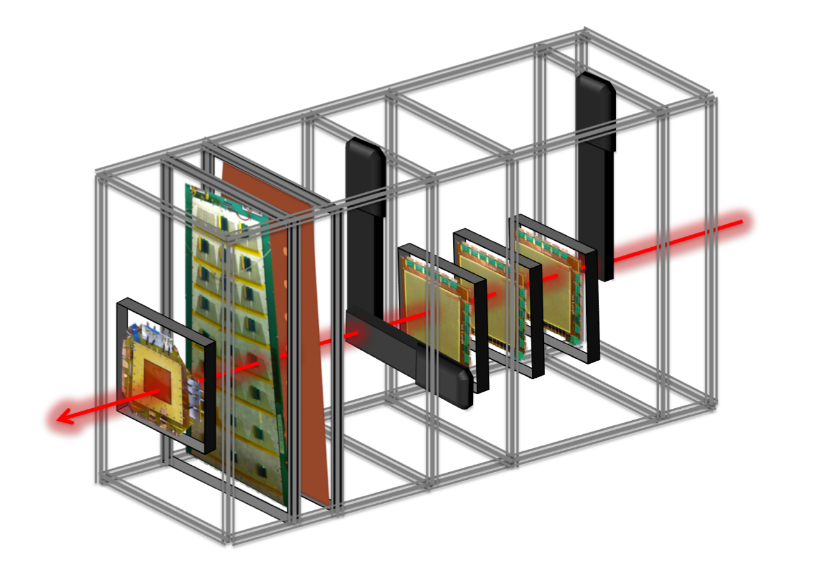
\includegraphics[width=0.95\textwidth]{figures/GEM/tbsetup.png}
%         \caption{Schematic view of the beam test set-up with the three square GEM hodoscope and the trapezoidal CMS GEM chambers}
%         \label{fig:tbsetup}
%     \end{center}
% \end{figure} 
\begin{figure}[!htbp]
\centering
% 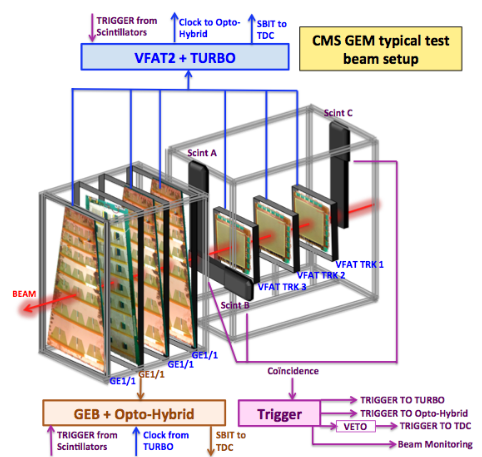
\includegraphics[width=0.95\textwidth]{figures/GEM/tb_exptsetup.png}
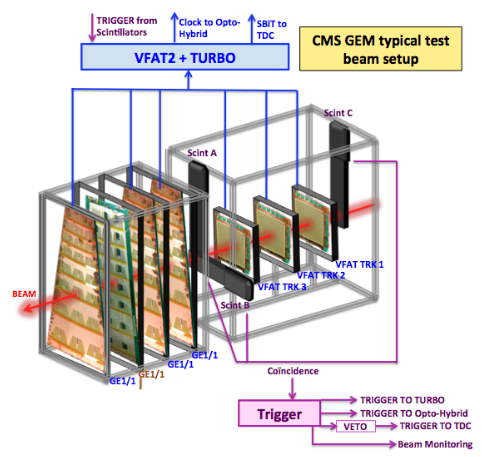
\includegraphics[width=0.75\textwidth]{figures/GEM/tb_exptsetup_copy.png}
\caption{Schematic view of the beam test set-up with the three tracking GEM detectors and a GE1/1 prototype.}\label{fig:daq}
\end{figure}
On detector electronics connects the output from the front-end ASIC (VFAT2) to the GEM readout board.
The VFAT2 chip is connected to the hybrids which are plugged into the connectors on the readout board.
%The trigger is generated using the coincidence of three photo-multiplier tubes with mounted scintillators. 
The analog pulses from the three scintillators, named S1, S2 and S3 are fed into discriminator for analog to digital conversion.
The discriminator output was provided into the logic coincidence (to generate event trigger) before being sent to the other DAQ systems (Figure.~\ref{fig:tbs}).
\begin{figure}[!htbp]
\centering
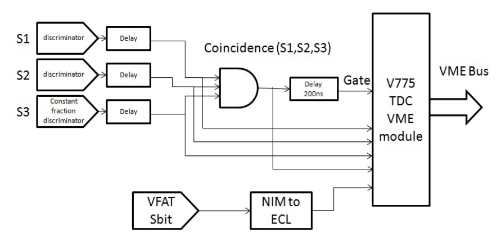
\includegraphics[width=0.95\textwidth]{figures/GEM/daq.png}
\caption{Perspective view of the experimental set-up used for performance measurement in the beam test studies. The trigger system is generated using the signal collected from three scintillators connected in coincidence.}\label{fig:tbs}
\end{figure}
% The active area of the GE1/1 detector is covered with readout strips located in the GEM Electronic Board. 
% The readout strips are taken out in 24 readout sectors (in ($\eta$,$\phi$) phase space).
% The data from each sector are collected using a VFAT2 front-end chip. 


%, with a tracker pitch of $0.4~mm$
\begin{figure}[!htbp]
\centering
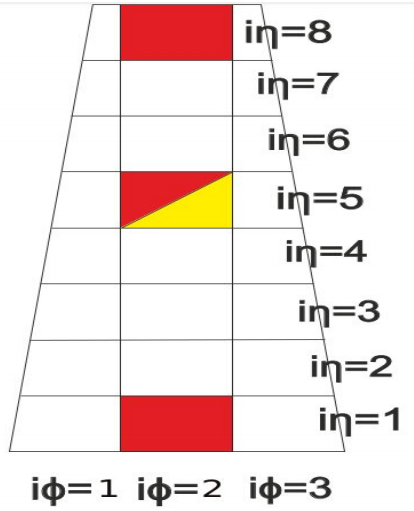
\includegraphics[scale=0.5,angle=90]{figures/GEM/GE11.png}
\caption{Different $(i\eta,i\phi)$ sectors of a full-size GE1/1 detector prototype. The red and yellow colour shows which sector of GE1/1 is exposed to the beam. Red sectors are collected with $Ar/CO_2/CF_4~(45/15/40)$ gas mixture while the yellow sectors are taken with $Ar/CO_2~(70/30)$ gas mixture.}
\label{GE1/1}
% THis is for beam test
\end{figure}
\subsection{Data Analysis} % (fold)
\label{sub:test_beam_analysis}
The raw data collected during these beam test campaign were in binary format. First, the raw data (binary information) is converted into the ROOT data format. ``\textit{\textbf{TURBO-SOFTWARE}}''~\cite{git-trubosoftware} package is used for data analysis framework, originally developed by TOTEM group, is used to perform this task. The output from TURBO-SOFTWARE data analysis consists of hit information for each strip from the detectors which are further used to reconstruct the particle tracks and clusters. 

A \textbf{hit} is defined when one or more strip of the VFAT chips surpass the threshold set on the readout chip. 
A \textbf{cluster} is defined as the number of adjacent fired strips along x or y-axis. The first step towards the track and cluster reconstruction is to discriminate the background tracks coming from detector noise (fake tracks) from the signal (muon) tracks. Once the fake tracks are removed from the collection, valid hits are used to generate tracks.

The hit profile and beam profile recorded in the tracker for one of the run are shown in Fig.~\ref{HitPosXaxis}~and~\ref{BeamProfile}.
From both hit profile and beam profile, one can see that the beam is point beam like a beam having a Gaussian spread, centred around (50,50), i.e., at the centre of the tracker.

This sorting is done by selecting events having only one cluster in each tracker. The cluster positions are fitted using a polynomial fit of order one and $\chi^2$ of the fit is recorded.
The event is discarded if the $\chi^2$ of the fit is greater than 10.
\begin{figure}[!htbp]
\centering
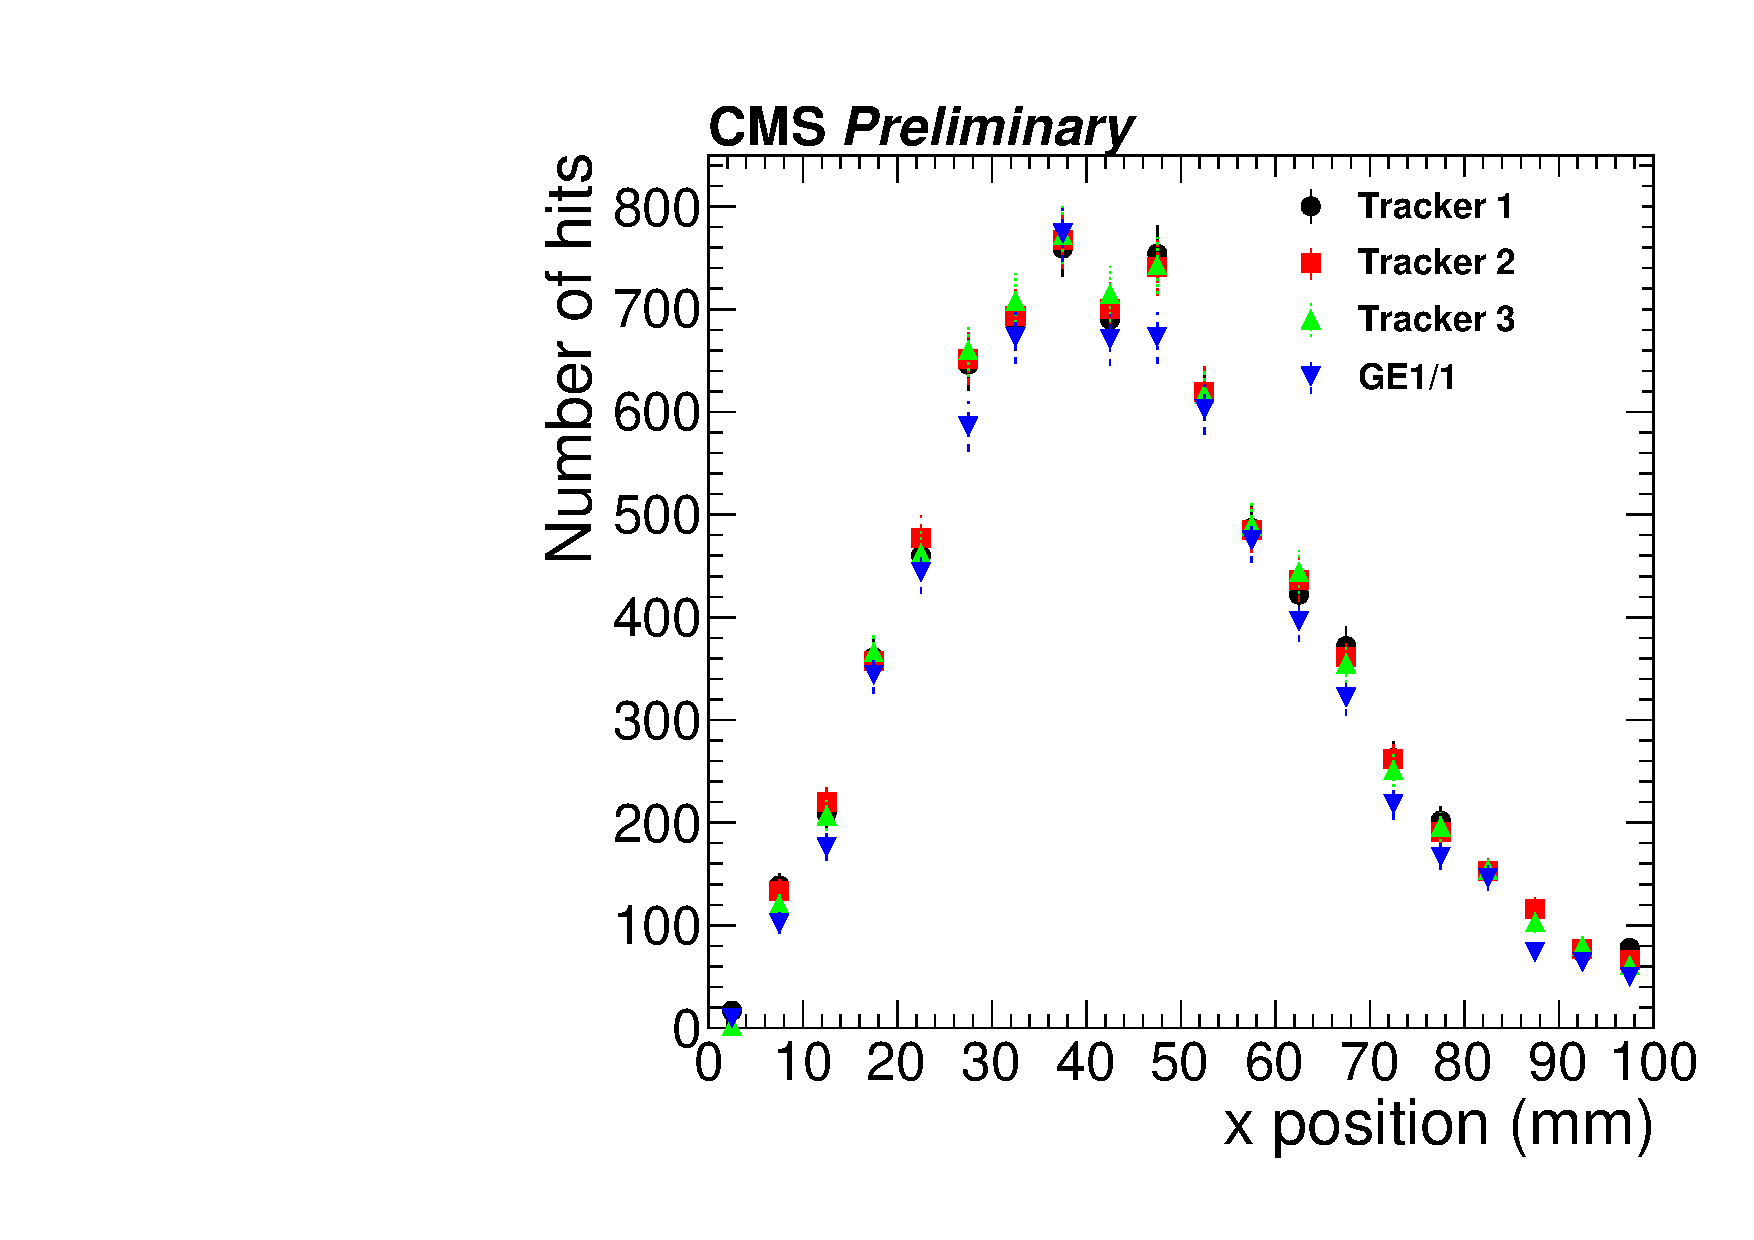
\includegraphics[width=0.45\textwidth]{figures/GEM/Tracker_Hit_position_Run1644_x.pdf}%
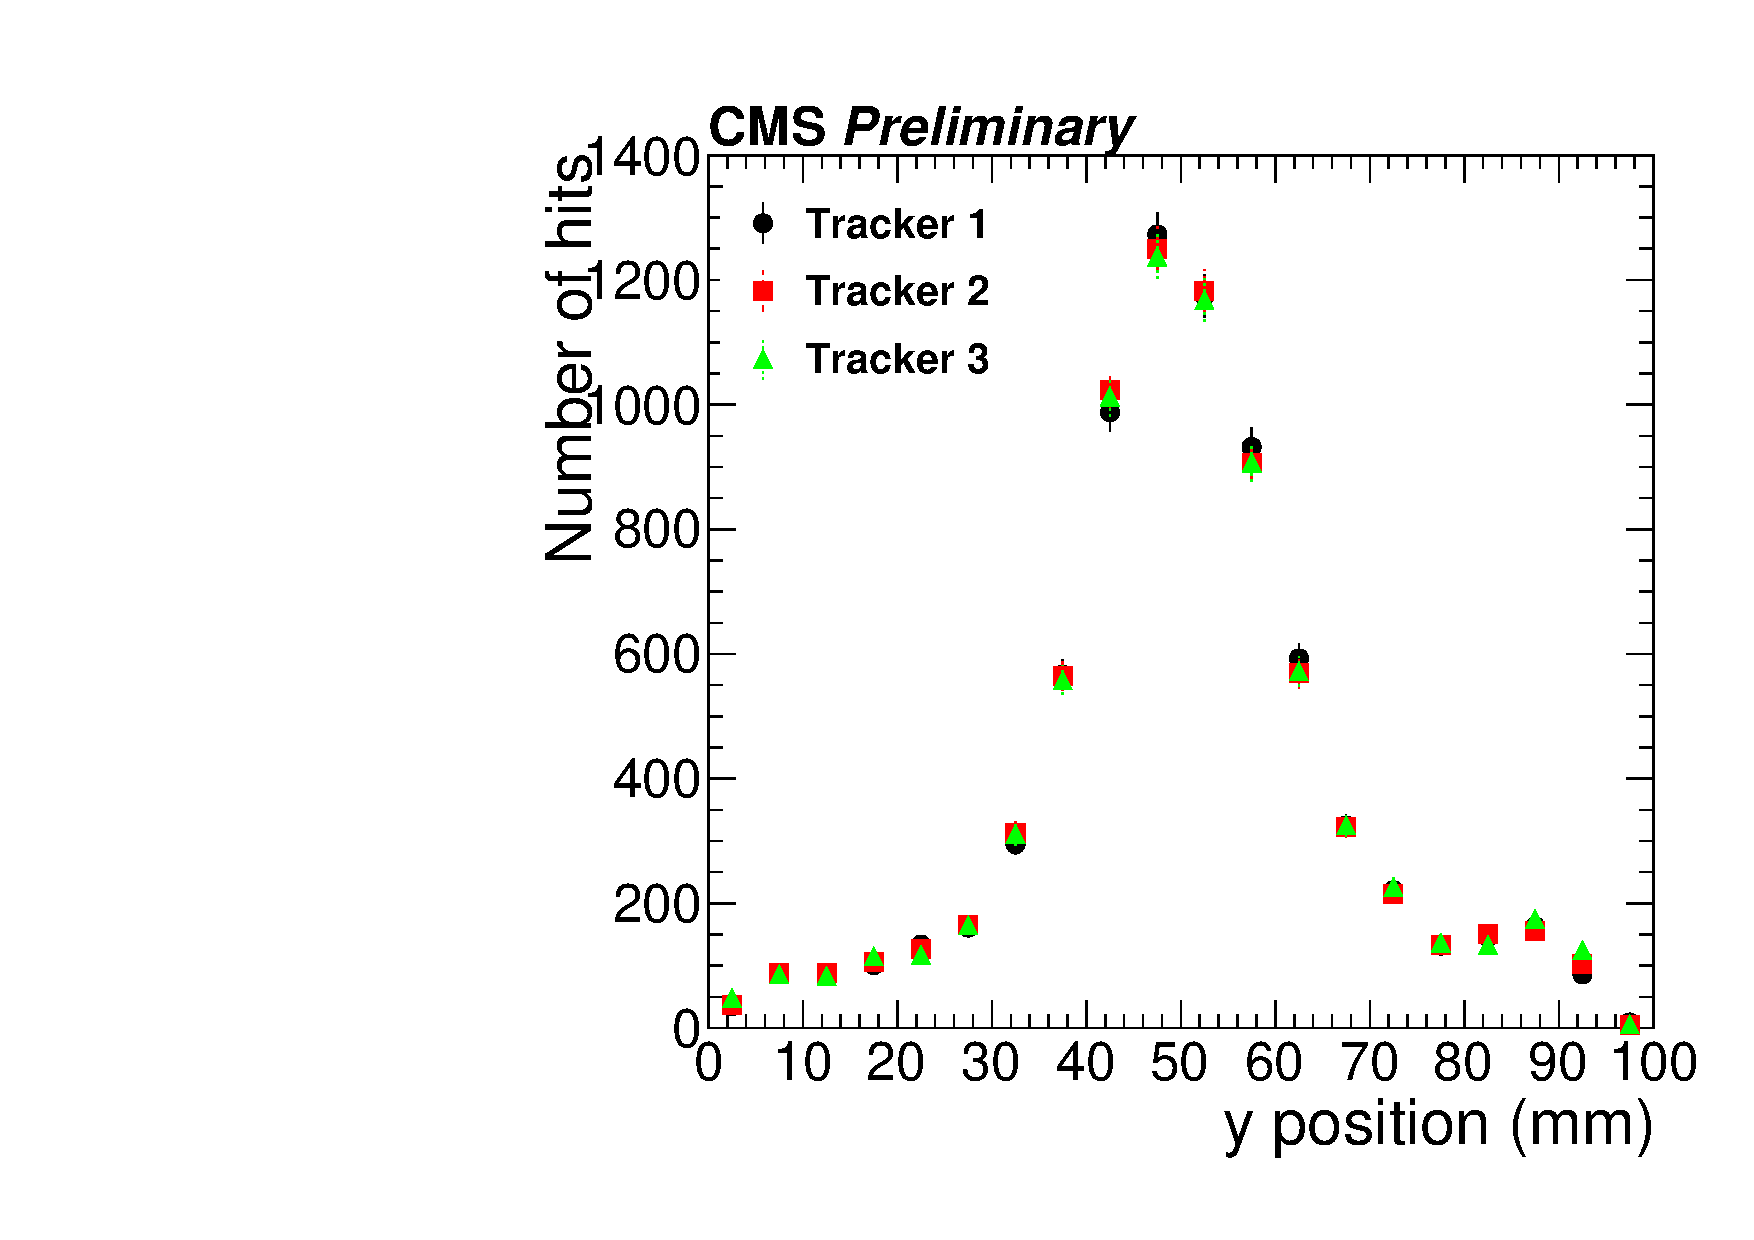
\includegraphics[width=0.45\textwidth]{figures/GEM/Tracker_Hit_position_Run1644_y.pdf}
\caption{Tracker hit distribution along x and y axis and GE1/1 hit distribution along y. This is plotted from one of run taken during test-beam.}
\label{HitPosXaxis}
\end{figure}
\begin{figure}[!htbp]
\centering
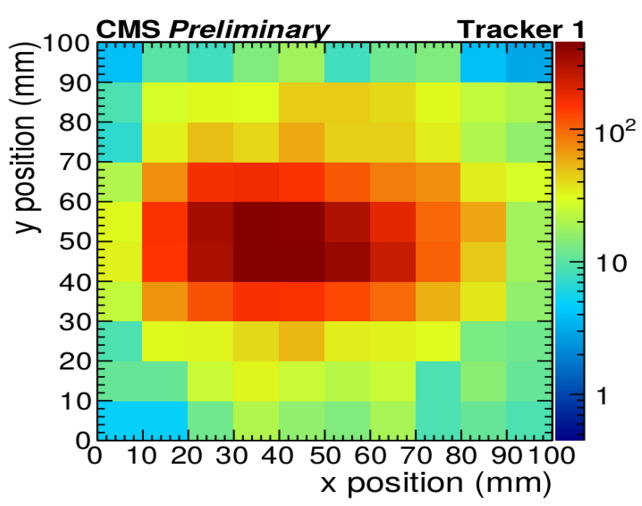
\includegraphics[width=0.5\textwidth]{figures/GEM/Selection_027.png}%
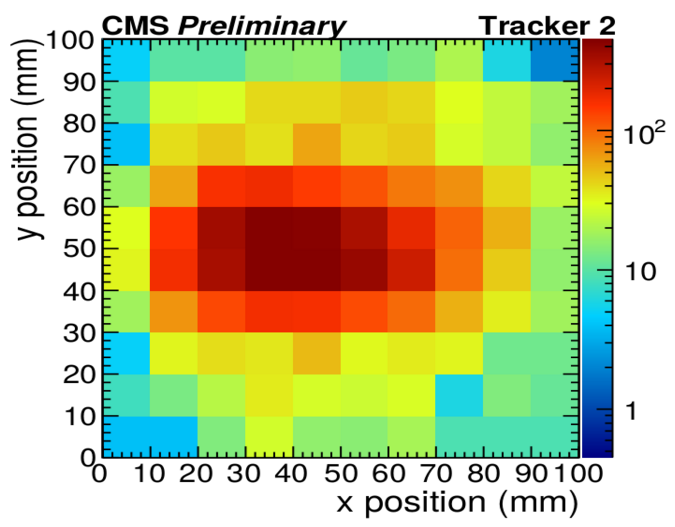
\includegraphics[width=0.5\textwidth]{figures/GEM/Selection_028.png}\\
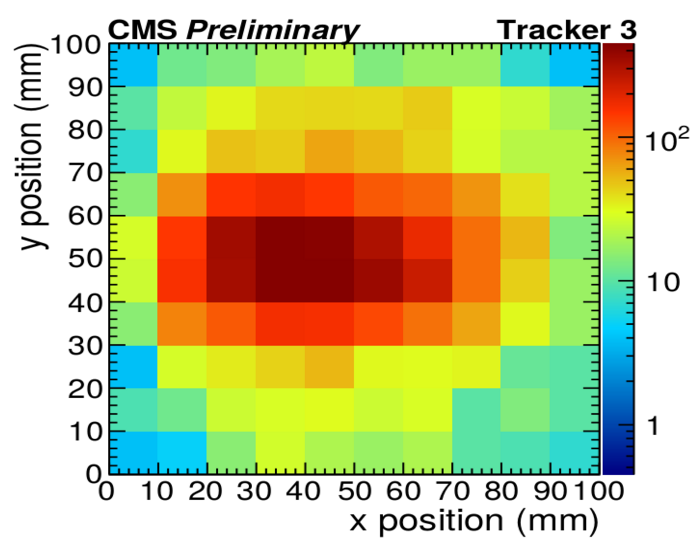
\includegraphics[width=0.5\textwidth]{figures/GEM/Selection_029.png}
\caption{2D- beam profile plot for the first, second and third tracker. The X and Y axis of the plots correspond to the distance (in mm) measured from the central position of the trackers in X and Y direction, respectively. The different colors in the color palette correspond to the number of hits registered in the detector at a particular (x,y) position.}\label{BeamProfile}
\end{figure}
% subsubsection track_reconstruction (end)
% subsection test_beam_analysis (end)

% subsubsection basic_results (end)ub
\subsubsection{Detector alignment studies}
Detector alignment is one of the core parts of the data analysis. 
For the efficient track reconstruction and for good tracking efficiency, it is necessary to align the detectors. Detectors can be aligned manually (online) and offline is software based.
During the beam test, the trackers and GE1/1's are aligned manually. Thus, one can achieve precession of up to few centimetres only.
Thus, it is always important to check the detector alignment using the software to achieve better efficiencies and spatial resolution.

The technique used for this purpose consists of the interposition along the trajectory of several detector planes where the particles pass through; from the interpolation of all these points can be reconstructed the trajectories followed by the particles.
In these environments one of the most important figure of merit of the detectors is the spatial resolution, that is the capability to reconstruct the crossing point of the particle.
The goal is to reduce the $\chi^{2}$ of the track fits, in order to improve track and quality eliminating or reducing bias in the detector data.
% Current detector alignment studies are performed using the data collected during 2014 the beam test of GEM detectors. 

\begin{figure}[htbp]
    \centering
    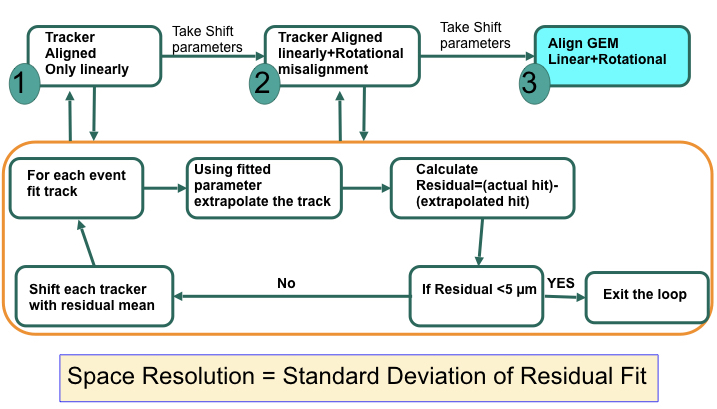
\includegraphics[width=0.95\textwidth]{figures/GEM/GEM_Alignment_FlowChart.jpeg}
    \caption{Flowchart illustrating the workflow of detector alignment algorithm.}
    \label{fig:alignment}
\end{figure}

\subsubsection{Linear and Rotational Alignment}
To measure the spatial resolution of GE1/1 detectors, these detectors aligned with respect to the tracker system.
This starts with the need to be mutual alignment of the three tracking detectors that have 2-D readout in the Cartesian coordinate system.
% The first step in the resolution measurement is an alignment of the three small tracking detectors that have a Cartesian X-Y strip readout.
% The trackers are first aligned with respect to each other in Cartesian coordinates.
The first alignment step is to shift each of the three tracking detectors iteratively in the XY-plane to make their origins coincide in the same line of sight.
% match with each other in that plane.
The initial shift parameters are the mean values from the position distributions  of X and Y axis.
During each iteration, a linear fit is performed to the hits position along X and Y direction from each tracker.
 % lines are fitted to the hits in X and Y.
% In this measurement study, residuals are histogrammed for each detector and the residual distributions are fitted with a double-Gaussian function.
Residuals are histogrammed for every detector and their distributions are fitted with a double-Gaussian function.
Ten percent of the residual mean value of each detector is taken as the shift parameter in the next iteration to avoid overcorrection.
This step is repeated until the resulting residual mean value converge towards zero.
% with iterations and provide a first coarse alignment.
This method provides a first coarse alignment.
In the second alignment step, we correct also for relative rotations of the tracking detectors around the beam axis in the XY-plane.
We again fit straight lines to the hit in X and Y direction and iterate through a succession of offsets and rotations around the beam axis relative to the first tracking detector.
Again this process is repeated until the residual means from the trackers are very close to zero and $\chi^2$ of the track fits is also observed at each iteration.
In each iteration, the detectors are first shifted and then rotated; then new residuals and rotation angles are calculated.
This process is repeated iteratively until the residual means from the track fits become less than 0.005 mm. Fig.~\ref{fig:alignment} shows the flow chart of the alignment algorithm.
Figure.~\ref{fig:alignmentIteration} shows the variation of track residuals for three trackers as a function of iteration number, with residual shifting to lower values progressively through iterations.
\begin{figure}[!htbp]
\centering
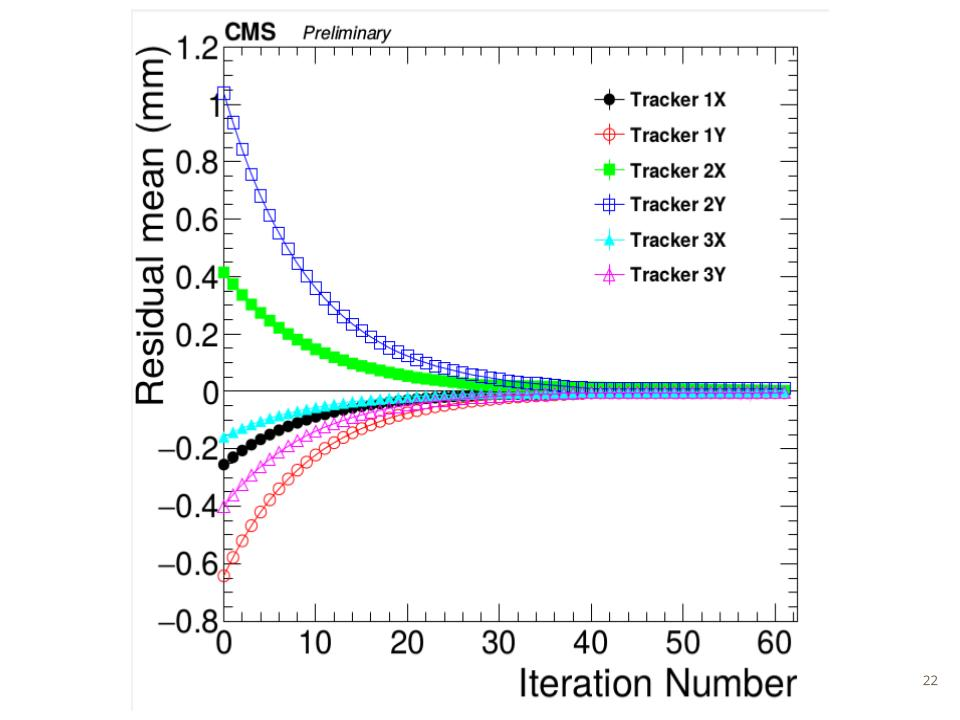
\includegraphics[width=0.65\textwidth]{figures/GEM/Tracker_iterative_alignment.jpg}
\caption{Variation of track residuals for three trackers with respect to the iteration number}\label{fig:alignmentIteration}
\end{figure}

\subsubsection{Alignment of GEM detectors w.r.t Reference Tracker}
Once the tracker alignment, the next step is to align trapezoidal GEM detectors with respect to the centre of the aligned tracker system.
A twofold iteration loop is used wherein the x-offset is kept fixed the y-offset is iterated over a set of values with a small iteration step.
The x-offset is also iterated over and corresponding to every single value of x-offset, the y-offset are iterated.
 % Y offset values with a small fixed step, ranging in a practical phase space.
% Then X offset is iterated and corresponding iterations are performed with Y offset.
For each value of (X offset, Y offset) pair, tracks are linearly fitted in the $\phi$ co-ordinate and the corresponding residuals are noted and used to align the detectors.

\subsubsection{Fiducial Area Selection} % (fold)
\label{ssub:fiducial_area_selection}
To have an efficient efficiency we should also define a fiducial area in which we are going to calculate the efficiency. We define the fiducial area as:

\begin{itemize}
        \item Only valid tracks are considered during this procedure, which are defined as the tracks having hits registered in all the three trackers.
        % \item For this only \textbf{valid tracks} are considered. Where the valid track is defined as the track that has hit in all three trackers.
        \item These valid tracks are then extrapolated to GE1/1’s. Only those tracks are finally selected for which the corresponding hit position in the GE1/1 has a residual value less than 5mm.
         % and accept that track as a hit in GE11’s if and only if the residual is less than 5 $mm$.
        \item The selected events are used to fill 2D histogram for different cases. The first histogram contains all those events that have a valid hit in the trackers only, as shown in Fig.~\ref{fig:fiducial_area_sel} (left). Another 2D histogram is filled with all those events where there are valid hits in all three trackers as well as in the GE1/1, as shown in Fig.~\ref{fig:fiducial_area_sel}(right). The ratio of the two histograms defined above is computed and is shown in Fig.~\ref{fig:fiducial_area_sel} (bottom)
        \item Finally, the region (0,80) in the ratio histogram where efficiency is maximum is considered as the fiducial region. This fiducial region is used for the efficiency calculation for GE1/1 detector.
\end{itemize}
Here, the calculated fiducial region is (0,80), which can be observed from Fig.~\ref{fig:fiducial_area_sel}(bottom).
\begin{figure}[htbp]
    \centering
    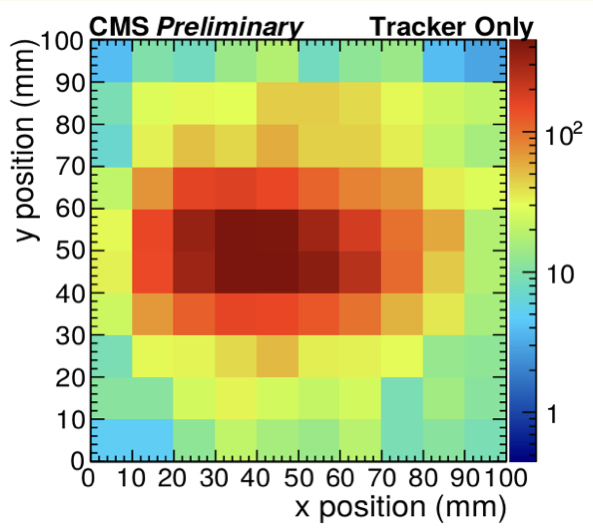
\includegraphics[width=0.45\textwidth]{figures/GEM/FiducialAreaCal_TrackerOnly.jpeg}%
    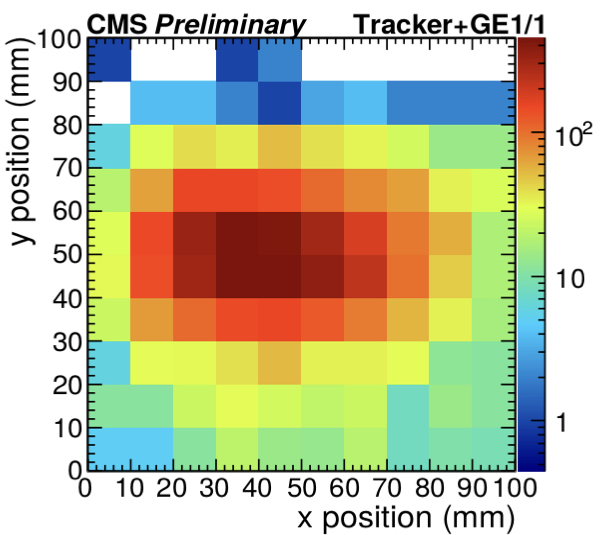
\includegraphics[width=0.45\textwidth]{figures/GEM/FiducialAreaCal_TrackerGE11.jpeg}\\
    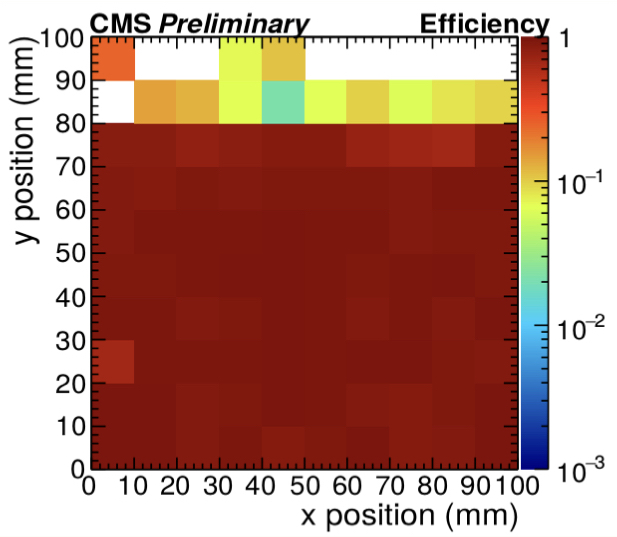
\includegraphics[width=0.55\textwidth]{figures/GEM/FiducialAreaCal_Selection.jpeg}\\
    \caption{2D distributions showing events with hits registered in the trackers (top left), events registered in three trackers and GE1/1's (top right) and the division of the two histograms used to define the fiducial region for GE1/1 efficiency measurements (bottom).}
    \label{fig:fiducial_area_sel}
\end{figure}
% subsubsection fiducial_area_selection (end)
\subsubsection{Efficiency Measurement}
Efficiency, $\epsilon$, for a GE1/1 detector for the current beam test set-up is defined as:
% Efficiency, $\epsilon$, is one of the most important parameters for the gaseous detectors. Here it is defined as 
\begin{equation}
\epsilon = \frac{N_{GE1/1+Trk}}{N_{Trk}}
\end{equation}
where $N_{Trk}$ is the number of reconstructed events with hits reconstructed in the three trackers
% by using a linear fit $y = mx + b$ fit to the tracker hit positions, in the tracker with normalized $\chi^2<10$.
and $N_{GE1/1+Trk}$ is the number of reconstructed events for which an actual hit is also found in the GE1/1 detector.
\begin{figure}[!htbp]
\centering
% 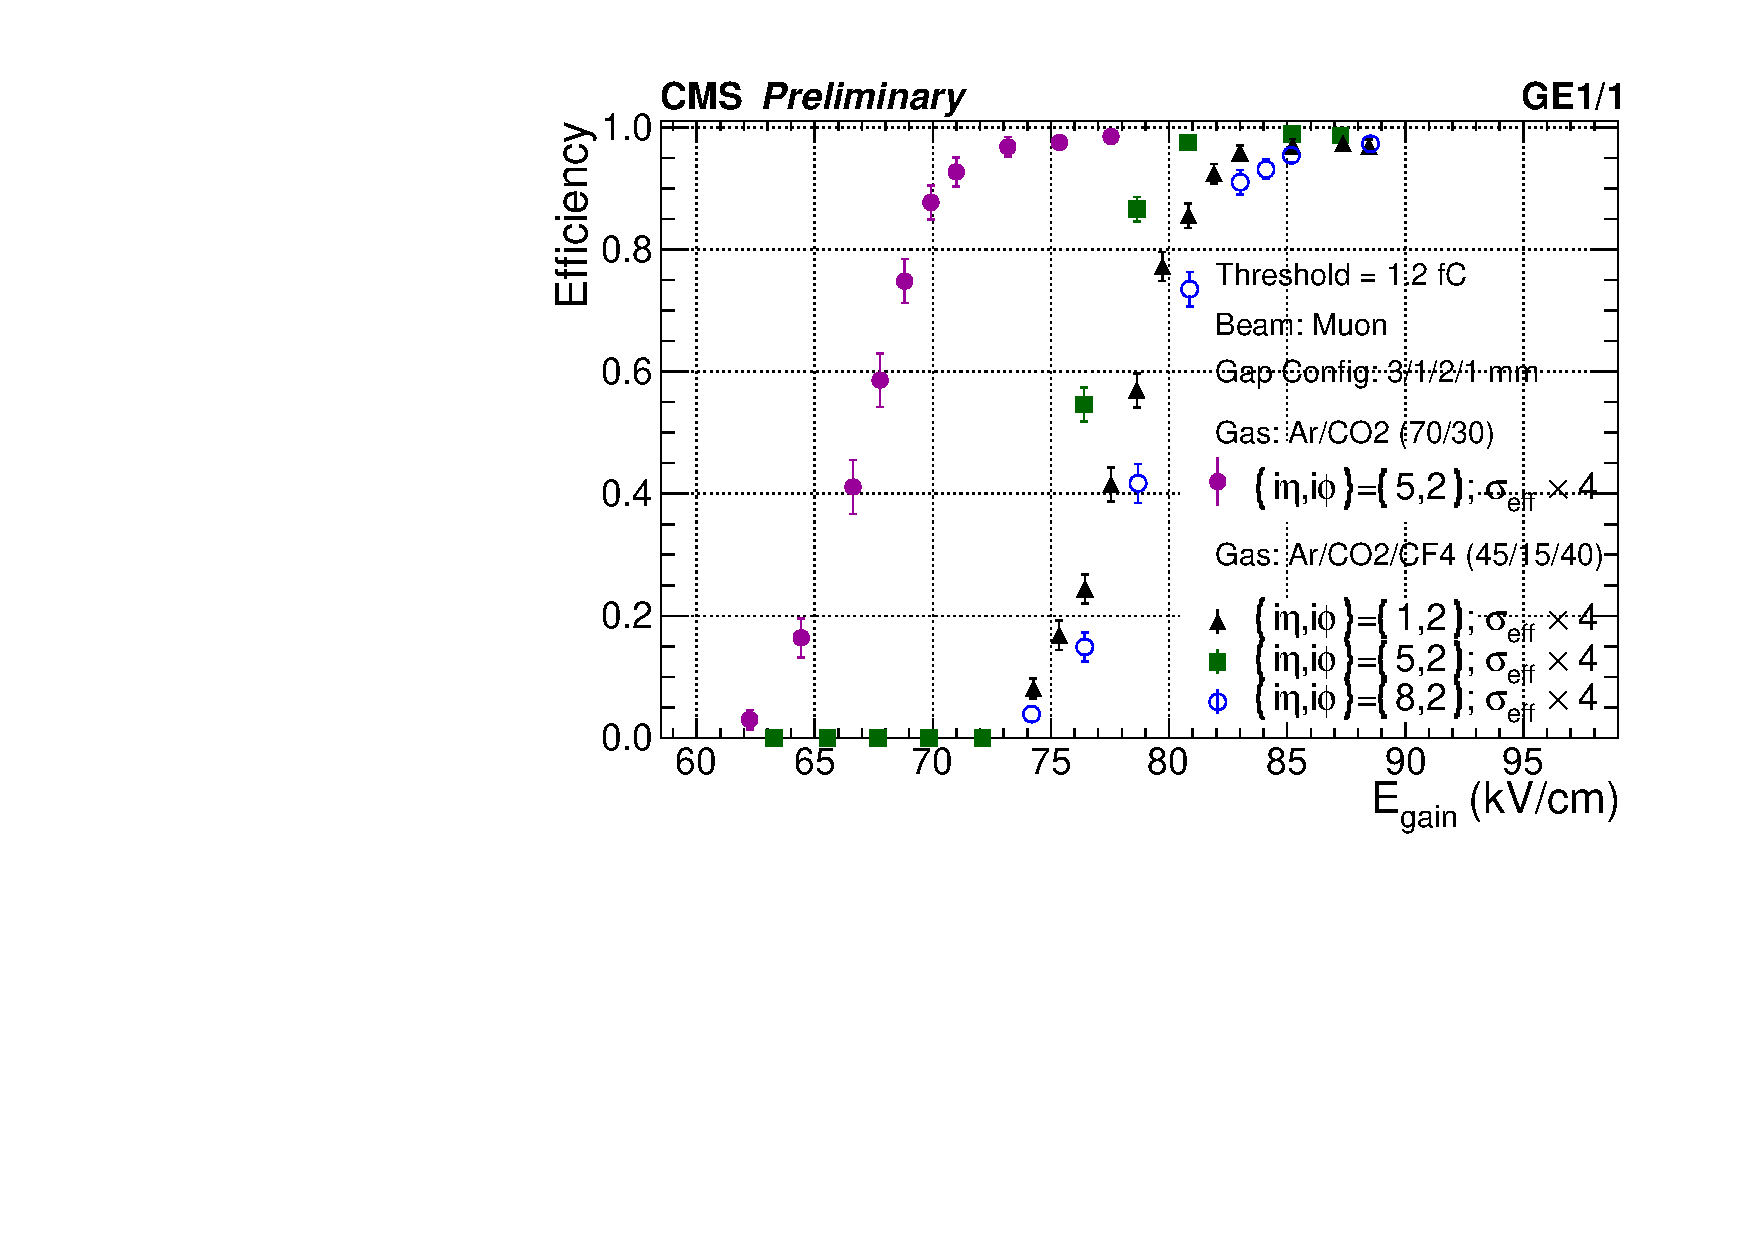
\includegraphics[width=3.5in]{figures/GEM/EfficiencyPlot_wrt_EGain_wError4times_2gas.pdf}
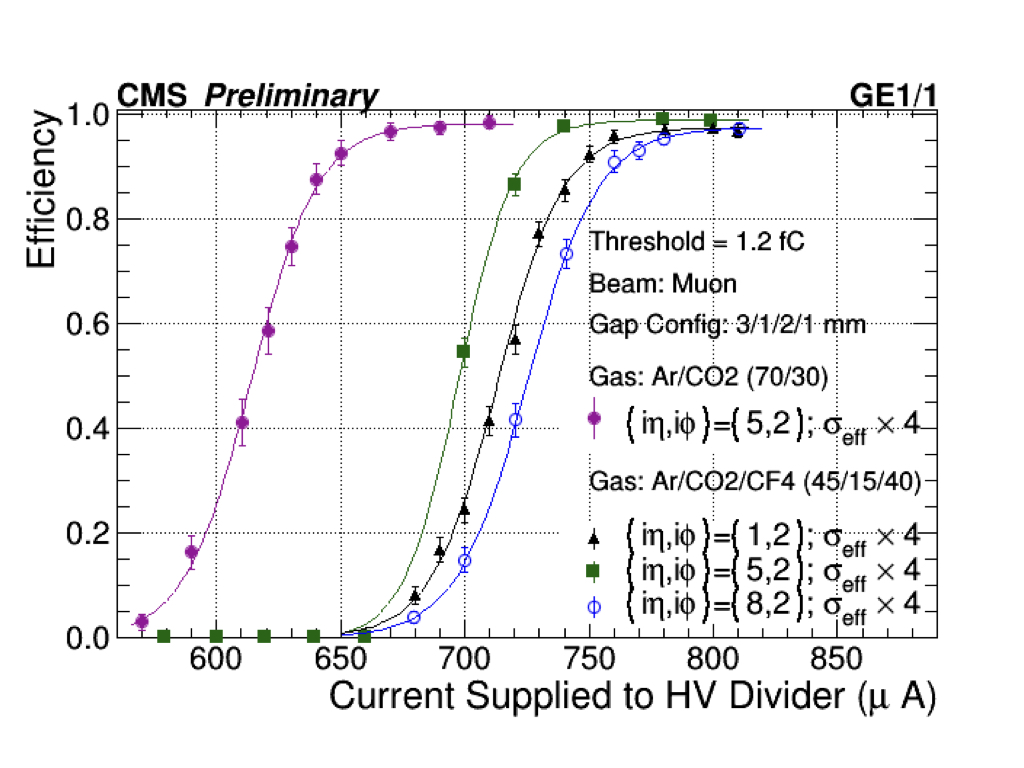
\includegraphics[width=0.75\textwidth]{figures/GEM/Efficiency_Current.jpeg}\\
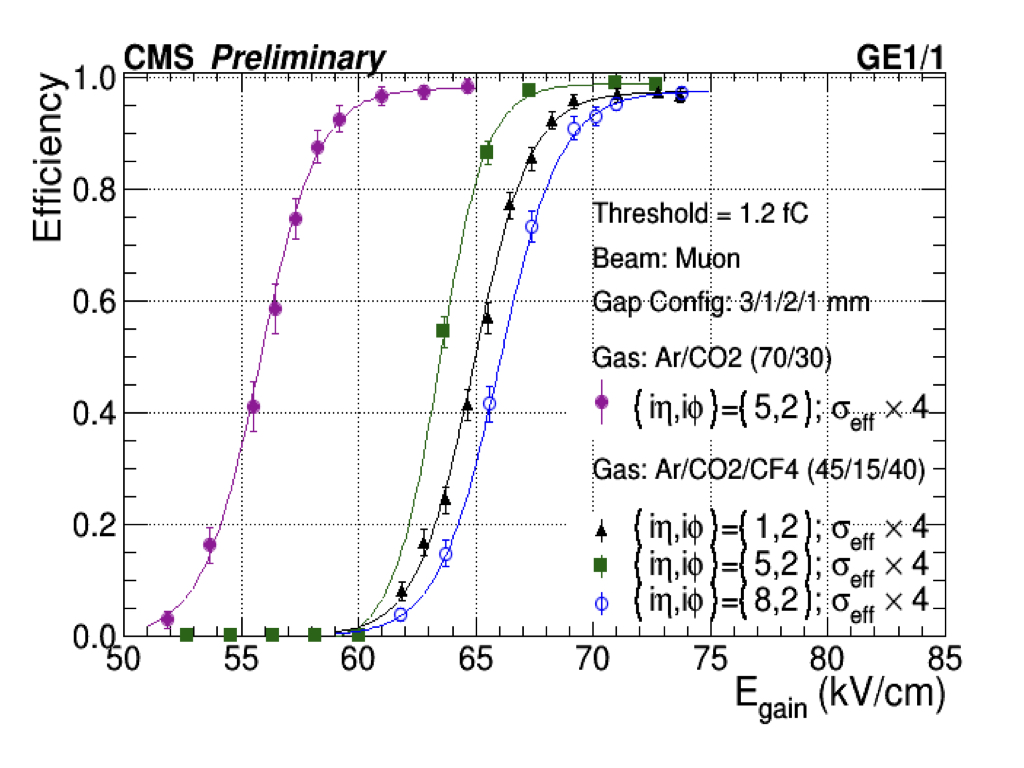
\includegraphics[width=0.75\textwidth]{figures/GEM/Efficiency_EGain.jpeg}
\caption{Efficiency with respect to $E_{gain}$ for two different gases and three different $(i\eta,i\phi)$ sectors.}
\label{Efficiency}
\end{figure}
% within $5~mm$ of an extra-plotted track.
% The fiducial region in which efficiency was calculated is (0,80) as shown in the previous section.
% We are showing here the efficiency as a function of current supplied to high-voltage divider as well as $E_{gain}$, Fig. \ref{Efficiency}. 
Detector efficiency is calculated as a function of current supplied to the high-voltage divider as well as $E_{gain}$ is shown in Fig.~\ref{Efficiency} where $E_{gain}$ is defined as
\begin{equation}
E_{gain} = \frac{I\times R_{avg}^{gap}}{D}
\end{equation}
where $I$ is current supplied to the HV divider, $R_{avg}^{gap}$ is the average gap resistance of GE1/1, and D is thickness of the GEM foil.
Here, the efficiency is fitted with the function defined as:
\begin{equation}
    \epsilon = \frac{\epsilon_{max}}{1+e^{s(HV-HV_{50\%})}}
\end{equation}
Where, $\epsilon_{max}$ is the maximum obtained efficiency, $HV_{50\%}$ is the applied HV (or current or $E_{gain}$) at which the efficiency is 50\% and $s$ is just a scale factor left floating for fit to determine. The fit parameters are shown in appendix~\ref{cha:efficiency_and_time_resolution_fit_parameters}.

Fig. \ref{Efficiency} shows the GE1/1 detection efficiency with two different gas mixtures $Ar/CO_2$ (70/30) calculated for sector $(i\eta,i\phi)=(5,2)$ and $Ar/CO_2/CF_4$ (45/15/40) for three different sectors $(i\eta,i\phi)=\{(1,2),(5,2),(8,2)\}$.
We achieved a very good efficiency of $\sim$ 98\% in all cases.
It should be noted that the efficiency curves for different gas mixture do not coincide because for a given high voltage operating point, the effective gain of detector with $Ar/CO_2$  mixture is approximately one order of magnitude higher than that for the $Ar/CO_2/CF_4$ mixture.
This implies that we can operate our detector without using $CF_4$ gas, which is non-eco friendly, without compromising with the efficiency.
      

\subsubsection{Time Resolution}
The time resolution is defined as the time taken by detector to generate a signal on the readout electrode after the passage of particle through it.
% The time resolution of a detector is defined as the minimum gate width necessary on the detection electronics for full efficiency.
Experimentally, the time resolution is the root-mean-square of the Gaussian distribution of the time taken by the particle to reach detector from the scintillator.
% Along with the fast 40MHz ($25~ns$) clock pulse has been used to cope with the LHC bunch crossing.
The detector time response is modelled as the Gaussian function, $f(t)$, convoluted with a square wave, $g(t)$, having a pulse length $f_{clk}=25ns$ (LHC clock frequency) to represent discrete sampling. 
The functions $f(t)$ is given by:
\begin{equation}
f(t) = Ae^{-\frac{1}{2}(\frac{t-t_0}{\sigma})^2}
\end{equation}
where A is amplitude of Gaussian function, $t_0$  is the mean value of Gaussian, and $\sigma$ is the standard deviation of Gaussian. And, $g(t)$ is given by
\begin{equation}
g(t) =
      \begin{cases}
              0, & \text{else} \\
              1, & \text{$-\frac{f_{clk}}{2}<t<\frac{f_{clk}}{2}$}
      \end{cases}
\end{equation}
where, $f_{clk}$ is the length of created 40MHz window.
The convolution of the two functions is given as
\begin{equation}
(f*g)(t) = A \cdot \sigma \sqrt{\frac{\pi}{2}}\Big(erf\Big(\frac{u_{+}}{\sigma\sqrt{2}}\Big)-erf\Big(\frac{u_{-}}{\sigma\sqrt{2}}\Big)\Big)
\end{equation}
% where $A$ is the amplitude of the Gaussian function, $\sigma$ is the standard deviation of Gaussian, and 
where, $u_{\pm}= t-t_0\pm\frac{f_{clk}}{2}$. 
The the experimental data is fitted with this convoluted function.
% From, the fit we extract the time resolution of the detector before the convolution.
The extracted time resolution as a function of $E_{drift}$ and current supplied to high voltage divider as shown in Fig. \ref{TimeResolution}. 

Here, the time resolution for the detector operated using gas $Ar/CO_2$ gas mixture is fitted using a polynomial of degree 2, while the one with $Ar/CO_2/CF_4$ gas mixture was fitted using the polynomial of order 6. Also, the fit parameters for each fit is given in appendix~\ref{cha:efficiency_and_time_resolution_fit_parameters}.

The time resolution with $Ar/CO_2$ (70/30) is higher for lower values of $E_{drift}$.
% However, for any given point on the $Ar/CO_2$ curve has a gain approximately one order of magnitude higher gain than the corresponding gain with $Ar/CO_2/CF_4$ (45/15/40).
This means that we are able to reach faster timing at lower gains with addition of $CF_4$ and it is important from the point of view of detector safety because this will allow us to operate the detector at lower gains, hence reducing the discharge probability.

\begin{figure}[!htbp]
\centering
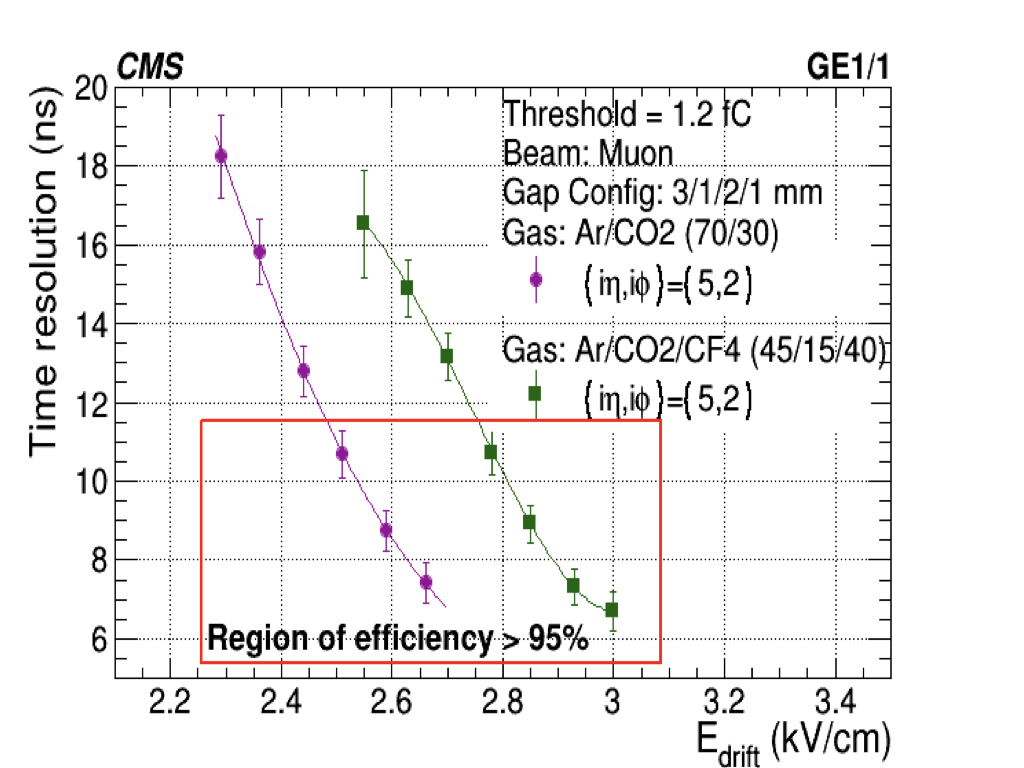
\includegraphics[width=0.75\textwidth]{figures/GEM/TimeResolution_Edrift.jpeg}\\
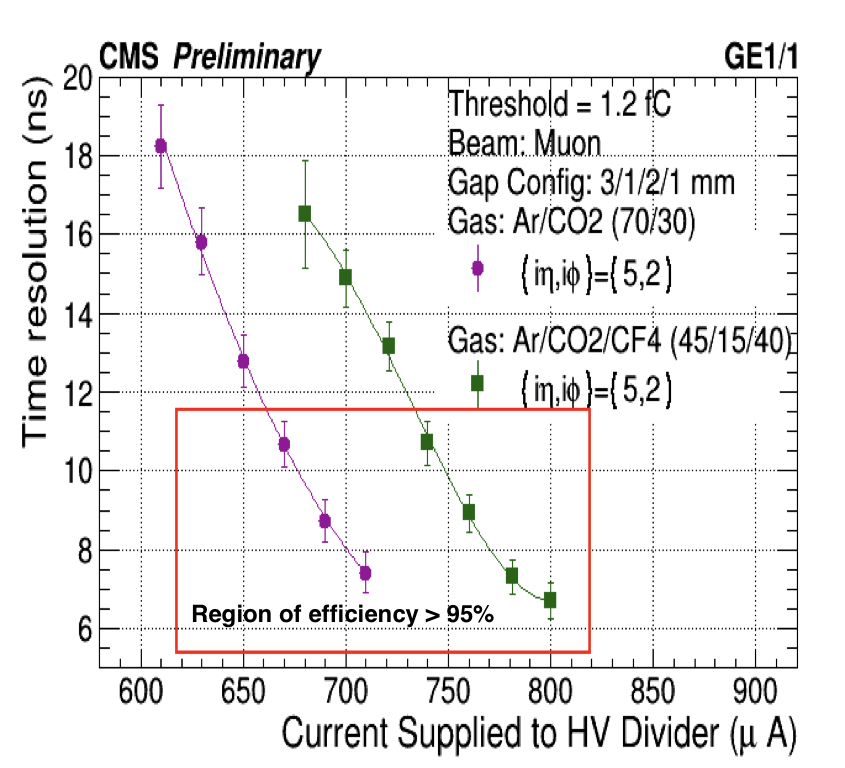
\includegraphics[width=0.75\textwidth]{figures/GEM/TimeResolution_Current.jpeg}\\
\caption{Time-resolution with respect to $E_{drift}$ (top) and current supplied to high voltage divider (bottom) for two different gas mixture.}
\label{TimeResolution}
\end{figure}
\begin{figure}[!htbp]
    \centering
    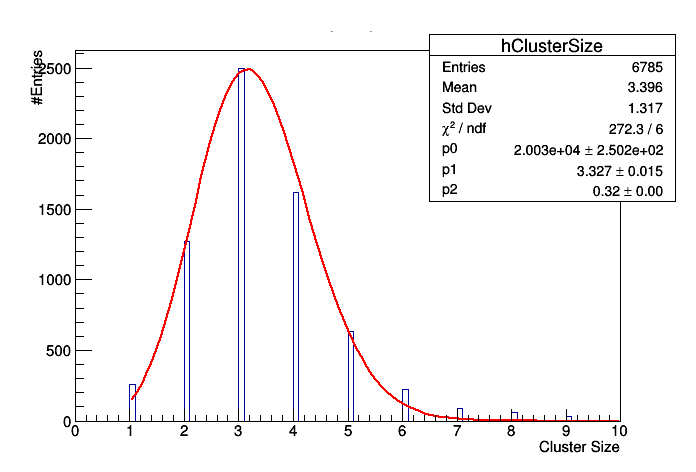
\includegraphics[width=5.5cm,height=6cm]{figures/GEM/Run1644.png}%
    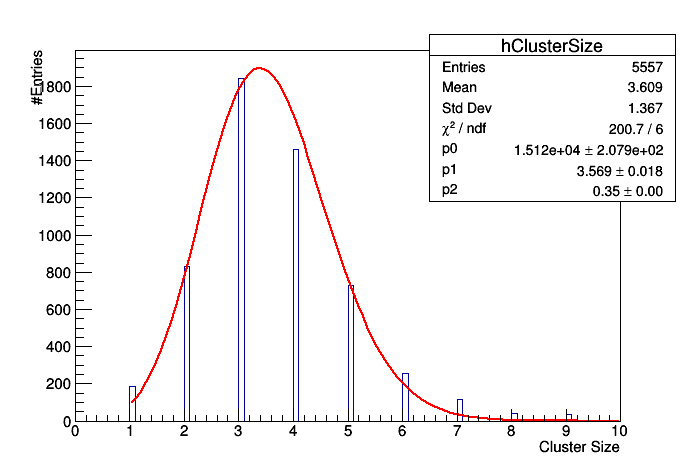
\includegraphics[width=5.5cm,height=6cm]{figures/GEM/Run1869.png}%
    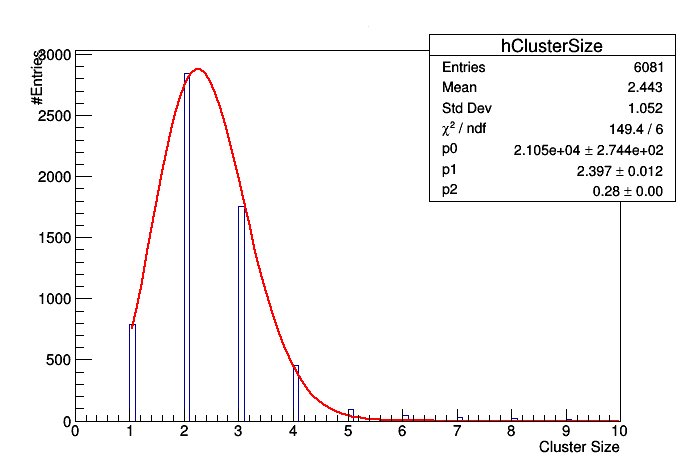
\includegraphics[width=5.5cm,height=6cm]{figures/GEM/Run2066.png}
    \caption{Cluster size distribution for GE1/1 detectors obtained during the beam test campaign: for run number 1644 in region ($\eta$, $\phi$) = (5,2) (left), for the Run number 1869 in region ($\eta$, $\phi$) = (8,2) (middle) and for Run number 2066 in region ($\eta$, $\phi$) = (1,2) (right).}
    \label{fig:CSDpoissonfunction}
\end{figure}
\begin{figure}[!htbp]
    \begin{center}
      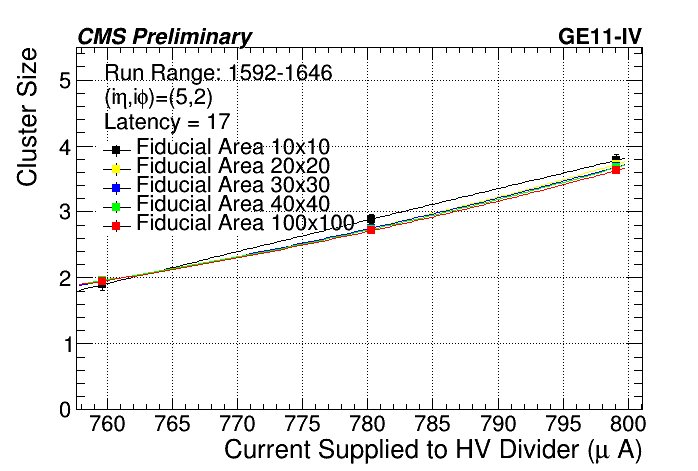
\includegraphics[width=5.5cm,height=6cm]{figures/GEM/CurrentvsClusterSizeR1592R1646.png}%
      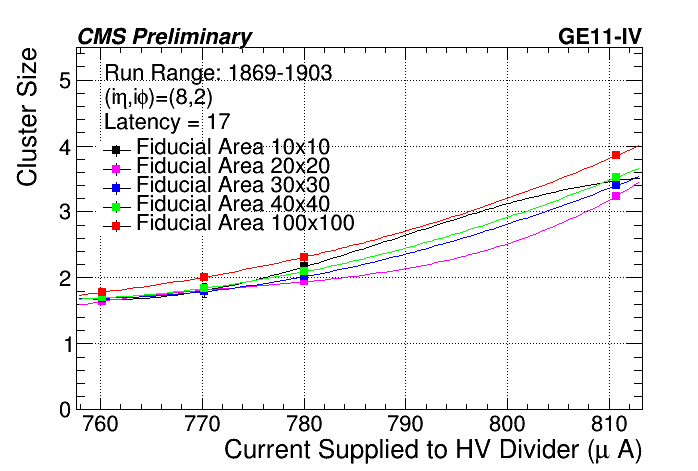
\includegraphics[width=5.5cm,height=6cm]{figures/GEM/CurrentvsClusterSizeR1869R1903.png}%
      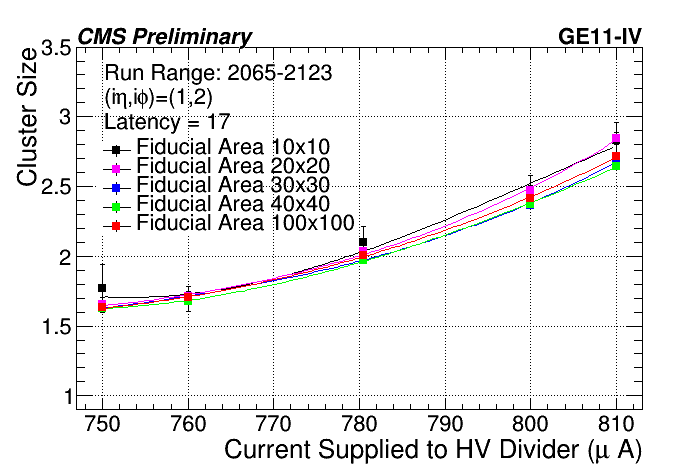
\includegraphics[width=5.5cm,height=6cm]{figures/GEM/CurrentvsClusterSizeR2065R2123.png}
    \end{center}
    \caption{Mean value of cluster size distribution at different current supplied to high voltage divider obtained during the beam test campaign: for 2014H4A which was taken for region ($\eta$, $\phi$) = (5,2) (left), for 2014H4C taken for region ($\eta$, $\phi$) = (8,2) (middle) and for 2014H4D taken for region ($\eta$, $\phi$) = (1,2).}
  \label{fig:CSDfiducialregion}
\end{figure}
\begin{figure}[!htbp]
   \begin{center}
     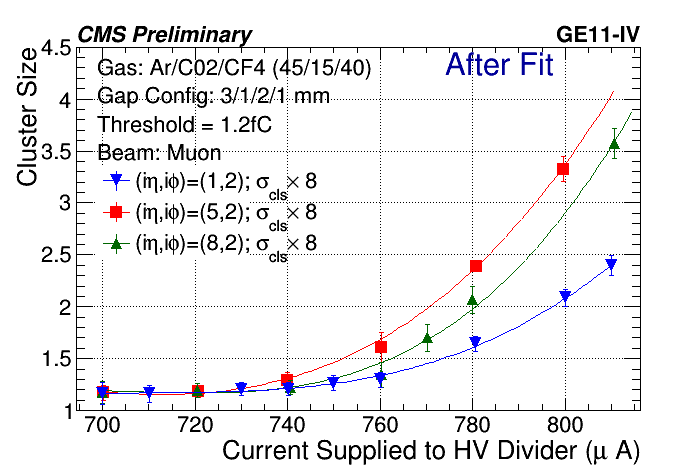
\includegraphics[width=6cm,height=6cm]{figures/GEM/CurrentvsClusterSizeAll3EtaPhi.png}%
     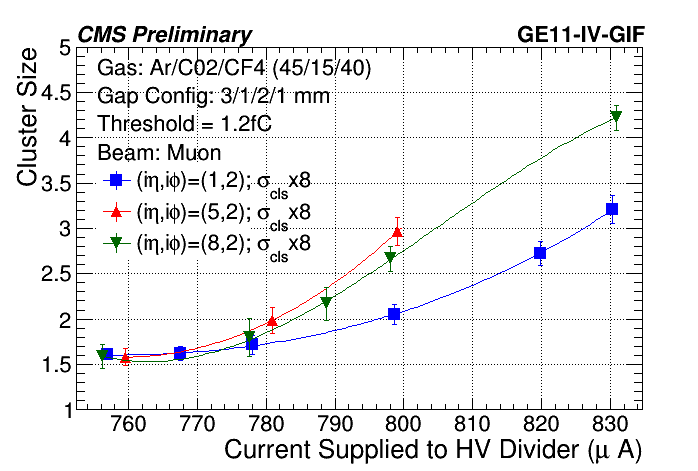
\includegraphics[width=6cm,height=6cm]{figures/GEM/CurrentvsClusterSizeAll3EtaPhiGE11IVGIF.png}
   \end{center}
   \caption{Cluster size distribution: Left - GE1/1-IV, Right - GE1/1-IV-GIF}
   \label{fig:CSDGE1/1}
\end{figure}


\subsubsection{Cluster Size Measurement}
To measure the cluster size of GE1/1, clusterization algorithm is used.
The basis of this algorithm is that we considered clusters if one or more continuous strips in GE1/1 are fired.
Three golden run ranges, with different eta sector, viz 2014H4A, 2014H4C and 2014H4D are studied.
The description of these runs is given in Table~\ref{tab:gemTBgoldenruns}.

To fit the cluster size distribution, Poisson function is used. Figure~\ref{fig:CSDpoissonfunction} shows the cluster size distribution for different ($\eta$, $\phi$) sector fitted using the Poisson distribution function.

% Study for the cluster size is done only for the three above mentioned golden run ranges.
Distribution is studied for different values of fiducial region and it is observed that the cluster size is independent of the fiducial region (Fig.~\ref{fig:CSDfiducialregion}).

Cluster size study distributions for the GE1/1-IV and GE1/1-IV-GIF are plotted as a function of current supplied to the high voltage divider and are shown in Figure~\ref{fig:CSDGE1/1}.
% Cluster size is taken with the Poisson fitting function. 
The cluster size is greater in ($\eta$, $\phi$) = (5,2) region for both the detectors due to the uniformity in readouts channels. As it is known that the GE1/1 $4^{th}$ generation prototype is suffered from the significant bending in the readout and drift PCB. This impacts GE1/1 properties like primary charge created, uniformity, transparency of bottom of third GEM foil, charge collection by the readout, etc. Thus, it is expected that that non-uniformity in the cluster size distribution in ($\eta$, $\phi$) sector (1,2), (5,2), and (8,2) is because of this. This issue is improved in the next version of GE1/1 prototype, known as GE1/1-V.
% subsection results (end)

% section gem_for_cms (end)

\section{Characterization and Production of GEM Foil} % (fold)
\label{sec:characterization_and_production_of_gem_foil}
Through the Transfer of Technology (TOT) agreement with CERN, Micropack Pvt. Ltd. (a Banguluru based company) signed an agreement for the development of GEM foil in India in association with the Indian Institution.
Micropack started producing the $10~cm~\times~10~cm$ GEM foils using the single mask technique, as  being used to produce GEM foils for GE1/1 detectors.
% But, after continuous effort and several trials they realized that single mask GEM foil production is the quite challenging method.
Soon it was realized that the production of GEM foil using the single mask technique is quite challenging and thus switched to the double mask production technique.
% and quickly they succeeded with this method. 
% They used the similar method used at CERN PCB workshop~\cite{DEOLIVEIRA2009}. 
Same production technique were adopted for the foil production as being done at the CERN PCB workshop~\cite{DEOLIVEIRA2009}.

Micropack used the Kapton foil having a thickness of 50 $\mu m$ with 5 $\mu m$ of copper coating on its either sides. Fig.~\ref{fig:Foil_and_Cone_a} shows the $10~cm\times10~cm$ GEM foil produced by Micropack and the cross-sectional view of its double conical hole is shown in Fig.~\ref{fig:Foil_and_Cone_b}.
\begin{figure}[!htbp]
    \centering
    \begin{subfigure}[b]{0.46\textwidth}
        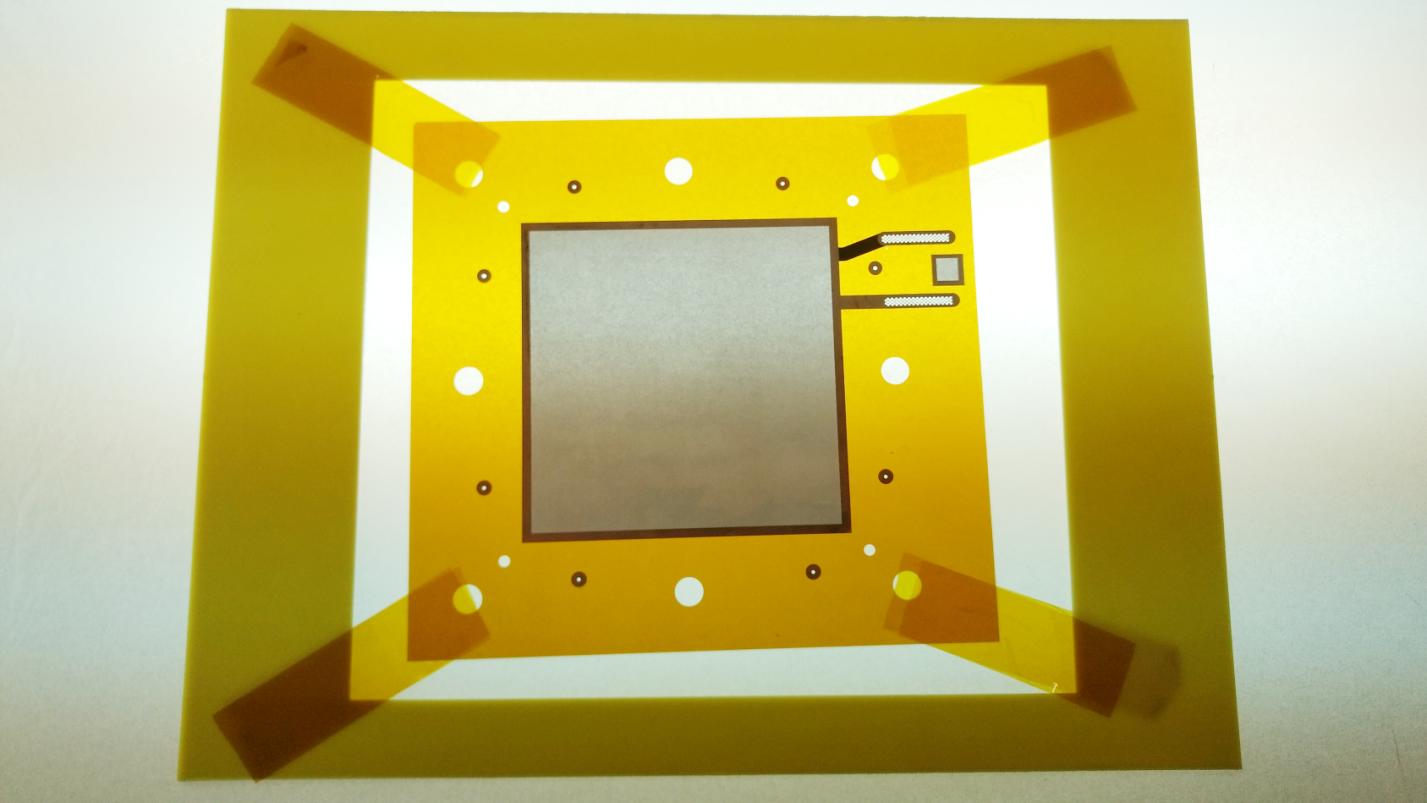
\includegraphics[width=6cm, height=4cm]{figures/GEM/figures/Foil_01.png}\qquad
        \caption{ }
        \label{fig:Foil_and_Cone_a}
    \end{subfigure}
    \begin{subfigure}[b]{0.46\textwidth}
        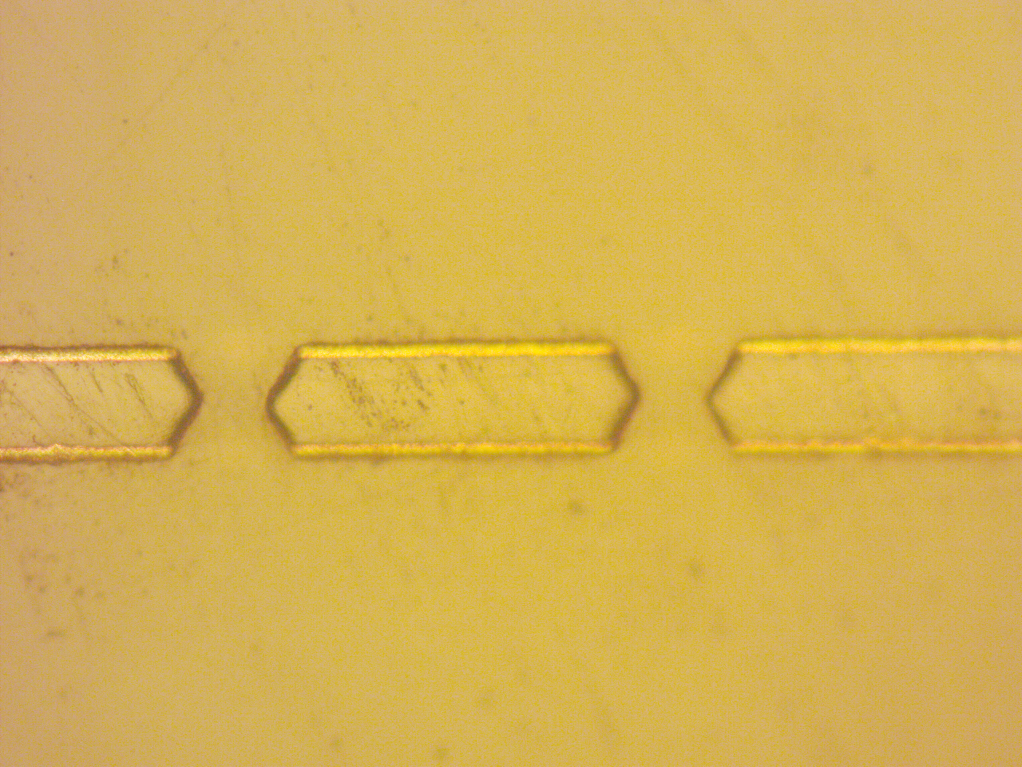
\includegraphics[width=6cm, height=4cm]{figures/GEM/figures/double_cone.png}
        \caption{ }
        \label{fig:Foil_and_Cone_b}
    \end{subfigure}
   \caption{(a) 10 cm $\times$ 10 cm GEM foil encapsulated in a frame and (b) Cross-sectional view of the foil showing the double cone structure of the engraved holes, developed by Micropack.} \label{fig:Foil_and_Cone}
\end{figure}

% To qualify the GEM foil commercially and scientifically reliable it has to pass some quality control test. For a GEM foil the general steps are listed below:
Before being used for the detector fabrication, the GEM foils required to pass certain quality control tests, which are listed below:
\begin{enumerate}
    \item Visual inspection
    \item Optical test, and 
    \item Electrical test
\end{enumerate}

% Before describing these three inspections one of the important tasks is that one should open/expose the GEM foil only in the clean room\footnote{Clean room is a specially designed room, maintained at extremely low level of particles per cubic meters, for a specialized industrial production or scientific research. For example, a ``\textit{Class-100}'' clean room is designed to never allow more than 100 particles (0.5 microns or larger) per cubic foot of air. ``\textit{Class-1000}'' and ``\textit{Class-10000}'' clean rooms are designed to limit particles to 1000 and 10,000 respectively.} of at least class 100 or better.
% As the typical size of GEM holes is 50 $\mu m$ and if it fills up with lots of dust then it will have a destructive discharge as soon as we connect it to the power.
% In Delhi University it was done in class 100 clean room installed with KANOMAX dust particle counter model 3887~\cite{KANOMAX-dust-particle-counter} which monitor particle count.

All these tests are required to be performed in the clean room\footnote{Clean room is a specially designed room, maintained at extremely low level of particles per cubic meters, for a specialized industrial production or scientific research. For example, a ``\textit{Class-100}'' clean room is designed to never allow more than 100 particles (0.5 microns or larger) per cubic foot of air. ``\textit{Class-1000}'' and ``\textit{Class-10000}'' clean rooms are designed to limit particles to 1000 and 10,000 respectively.} of at least class 1000 or better.
This is done to avoid the filling up of GEM foils with dust particles.
Even a small amount of dust inside the GEM holes could lead to a destructive discharge thereby destroys the whole foil.
At Delhi University the GEM foils are handled in the clean room of class 100. It is installed with KANOMAX dust particle counter model 3887~\cite{KANOMAX-dust-particle-counter} which continuously monitors the particle count inside the clean room.
Also, the clean room is equipped with a dehumidifier for humidity control.


\subsection{Visual Inspection} % (fold)
\label{sub:visual_inspection}
At first one has to inspect visually the GEM foil for any dust or defects visible to the naked eye.
GEM foils are cleaned using the adhesive rolled as shown in Fig.~\ref{fig:adhesive_roller} to remove dust particles.
% At first one has to inspect visually for dust particles and major defects visible to the eye.
% If things seem fine then one has to clean it using the adhesive roller, as shown in Fig.~\ref{fig:adhesive_roller}.
\begin{figure}[htbp]
    \centering
    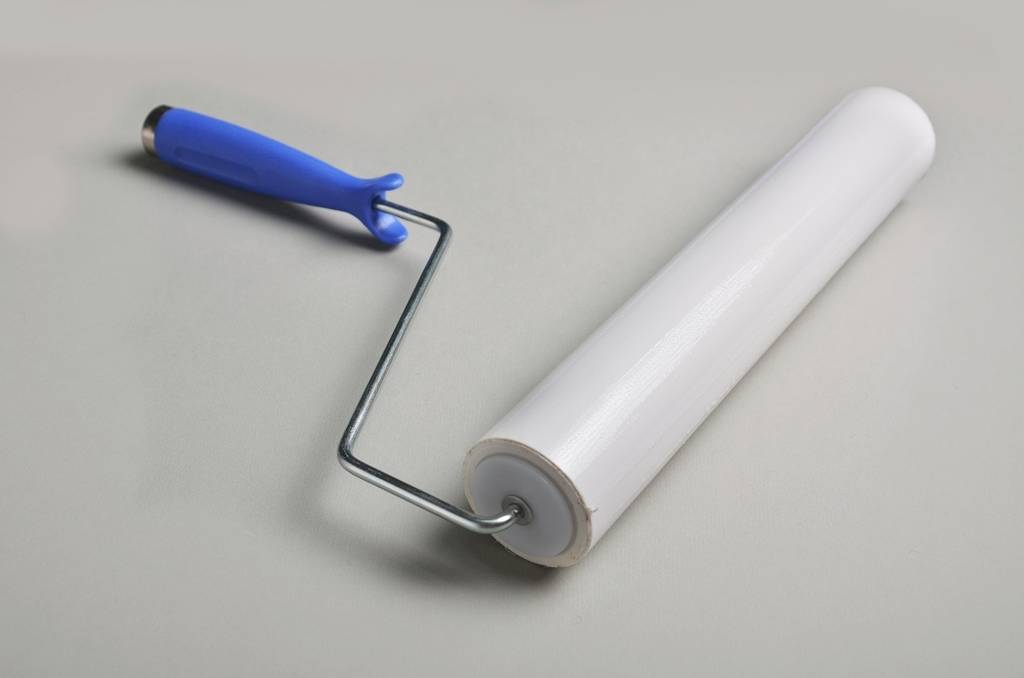
\includegraphics[width=0.55\textwidth]{figures/GEM/Adhesive_roller.jpg}
    \caption{Adhesive roller used for the cleaning of GEM foil.}
    \label{fig:adhesive_roller}
\end{figure}
% subsection visual_inspection (end)

\subsection{Optical Test} % (fold)
\label{sub:optical_test}
Optical test is carried out to check the GEM foil for any:
% Using an optical test we will try to find out:
\begin{itemize}
    \item microscopic defects, not visible to the eyes and
    \item to measure the inner and outer hole diameter and the pitch size.
\end{itemize}
The motivation to perform the optical test is following:
\begin{itemize}
    \item The foil defects such as the over-size hole, missing hole, excess etching, etc could degrade the performance of foil and thus the overall detector efficiency.
    % will degrade the performance of foil locally.
    \item As the gain of the detector depends on the diameter of the hole and thickness of the foil (as shown in Fig.~\ref{fig:gain-vs-holediameter}).
    Thus, it is necessary to check their dimensions.
    % So, it will help us to understand the performance of GEM foil such as gain, etc at a later stage.
\end{itemize}
\begin{figure}[htbp]
    \centering
    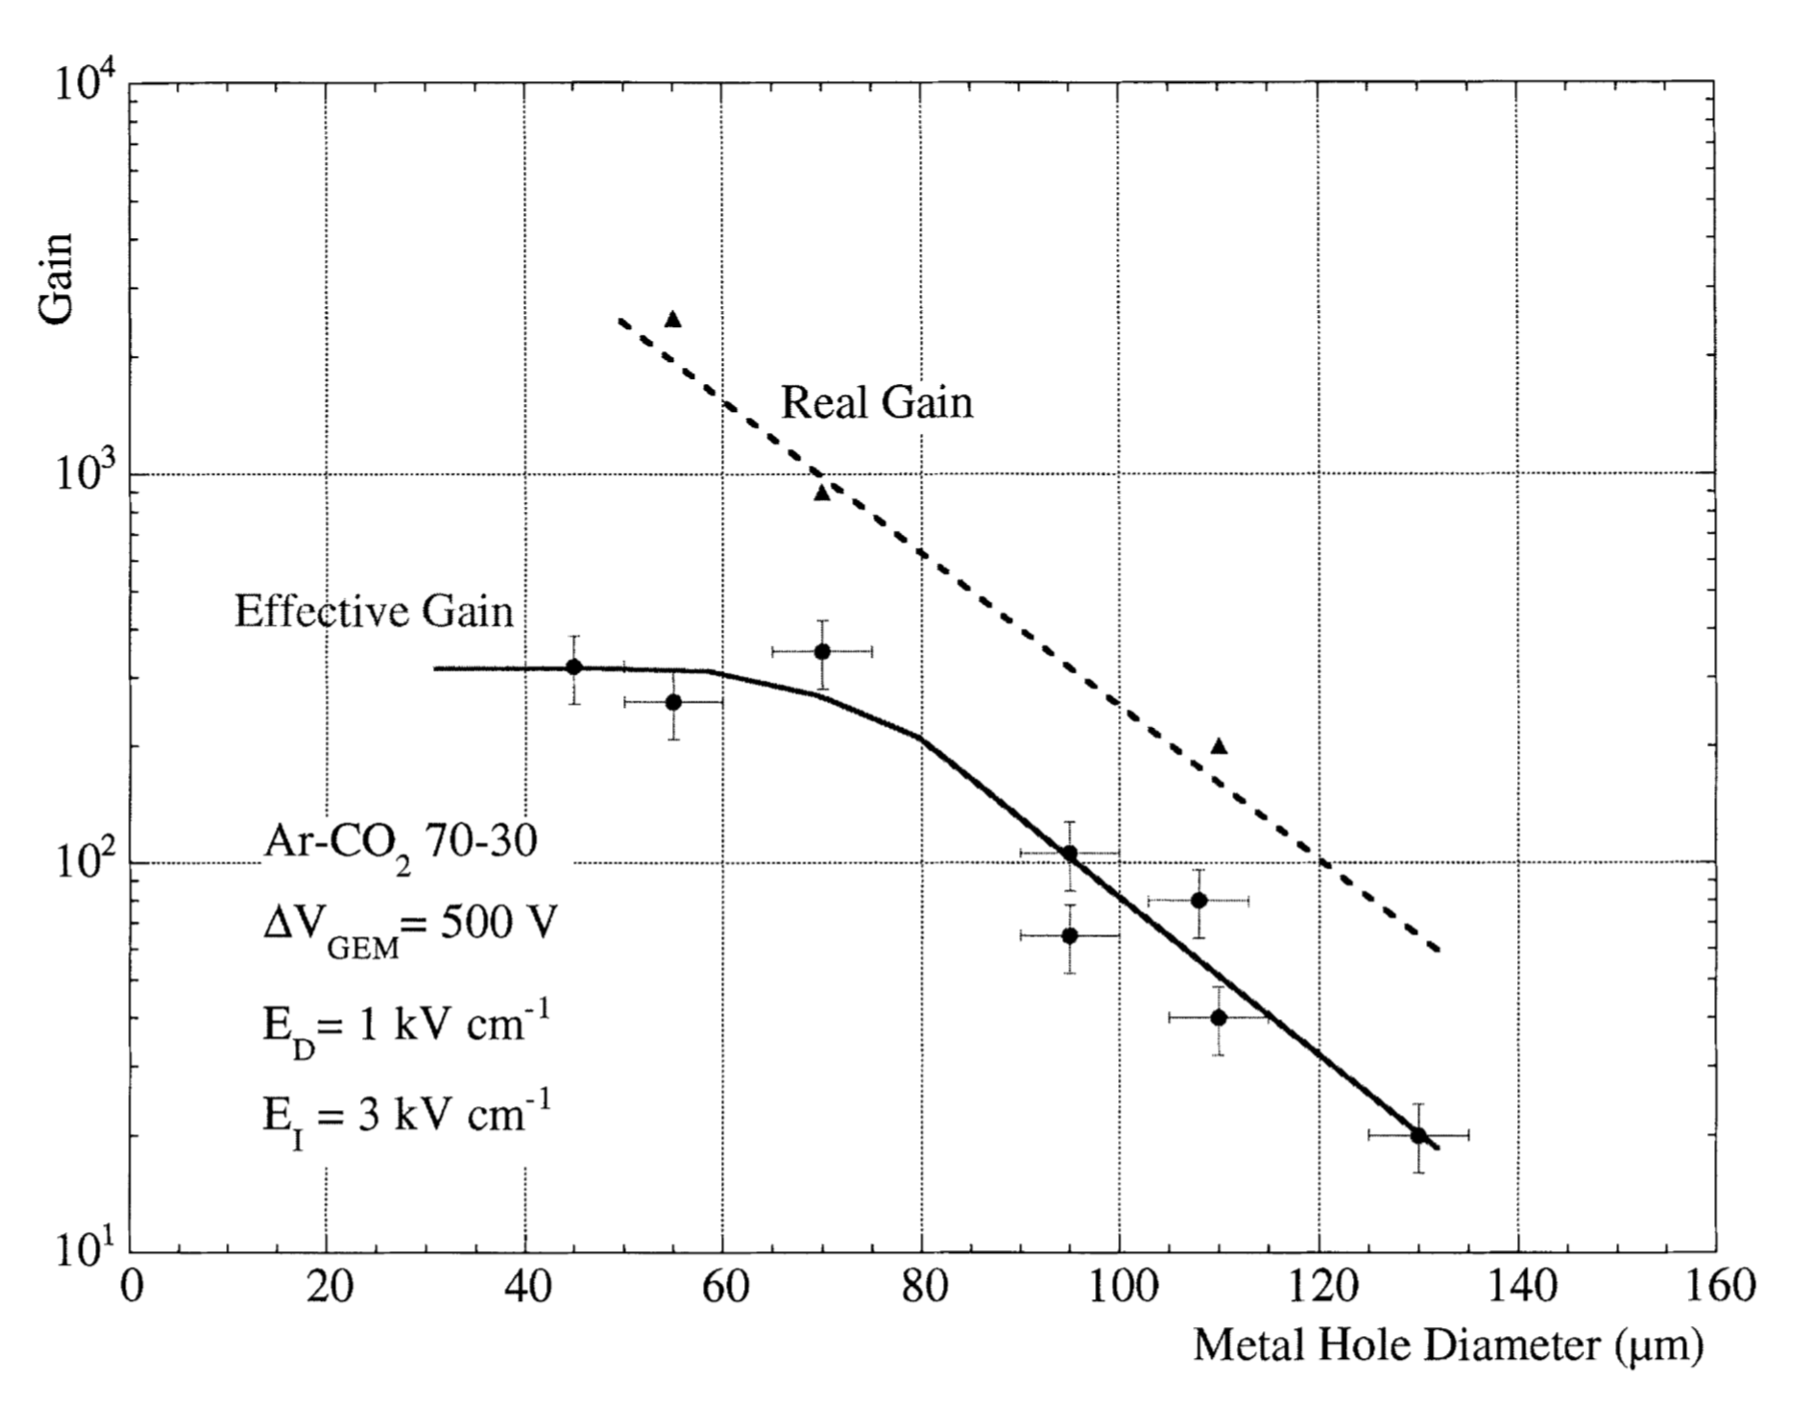
\includegraphics[width=0.65\textwidth]{figures/GEM/Gain_Vs_Hole_Diameter.png}
    \caption{Real gain and effective gain variation with GEM hole diameter~\cite{Bachmann1999} having a foil thickness of 60 $\mu m$ (= 50 $\mu m$ + 5$ \mu m$ + 5 $\mu m$). As the hole diameter decreases the effective gain increases till 70 $\mu m$ after that it reaches saturation. This is due to loss of generated electrons in the avalanche to the bottom of the GEM electrode when hole diameter is reduced below the foil thickness.}
    \label{fig:gain-vs-holediameter}
\end{figure}
To check any defects and to measure the hole-size and pitch for a GEM foil several methods have been developed using an automated 2D-CCD scanner~\cite{Posik2015, Becker2006}. 
However, we used a different technique.
We divided the GEM foil into several sectors and captured a high-resolution picture using the AF-S Micro Nikon 40 mm 1:2.8G lens.
We used a softbox ($1~m~\times~1~m$) light source for uniformly illuminating the GEM foil.
A sketch of the set-up is shown in Fig.~\ref{fig:Optical_Sketch}.
\begin{figure}[!htbp]
    \centering
    %\begin{subfigure}[b]{0.7\textwidth}
        %\includegraphics[width=12cm, height=8cm]{figures/GEM/figures/NIMA_paper_Images001.jpeg}
        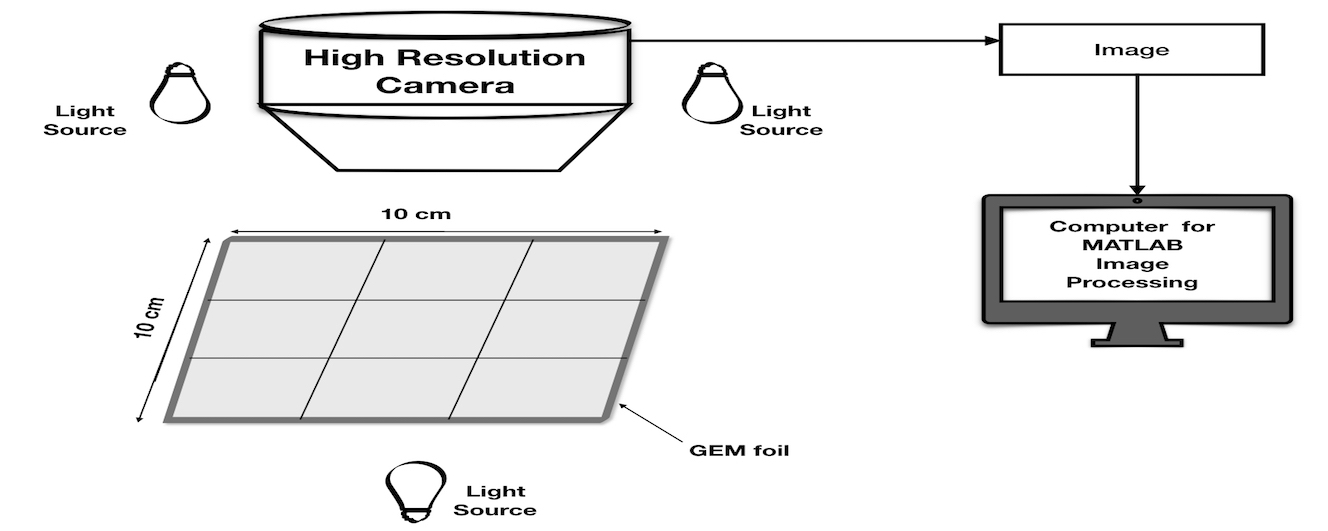
\includegraphics[width=12cm, height=8cm]{figures/GEM/figures/2.jpeg}
        %\includegraphics[width=9cm, height=8cm]{figures/GEM/figures/Optical_Sketch.png}
    %    \caption{ }
    %\end{subfigure}
   \caption{Sketch of the set-up used for optical measurements of the GEM foil.}   \label{fig:Optical_Sketch}
\end{figure}
Fig~\ref{fig:Optical_01} shows the found defects in the considered GEM foil.
Also, the observed number of defects are shown in Fig.~\ref{fig:Optical_04}.
% A total of 785 defects were found in the GEM foil out of total 600,000 holes in one GEM foil.
Out of 600,000 holes in the GEM foil, defects were found in 785 holes, i.e, 0.13\% of total holes are defected.
% Thus there is approximately 0.13\% of defects are there.
Also, similar number of defects were observed in other two GEM foils.
% Thus, the local effects in the GEM detector performance should be almost negligible due to the GEM foil defects.
The resulting local effects in the GEM foil due to these small fractions of defected holes are not expected to deteriorate the overall performance of the GEM detector.
\begin{figure}[!htbp]
    \centering
    \begin{subfigure}[b]{0.29\textwidth}
        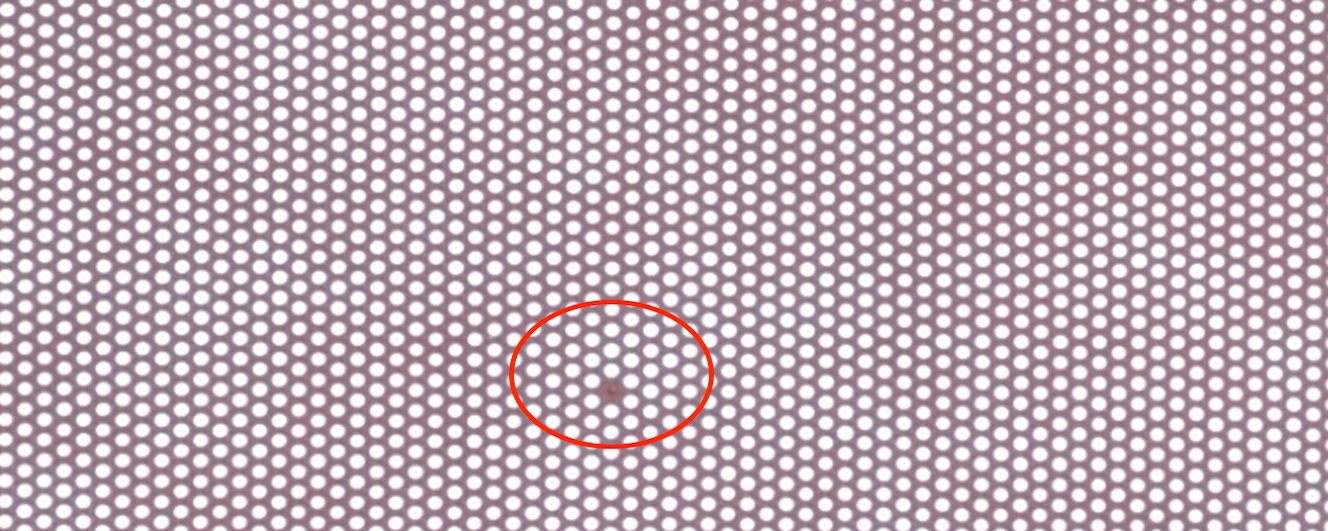
\includegraphics[width=4cm, height=3cm]{figures/GEM/figures/3a.jpg}
        \caption{ }
        \label{fig:O_4a}
    \end{subfigure}
    \begin{subfigure}[b]{0.29\textwidth}
        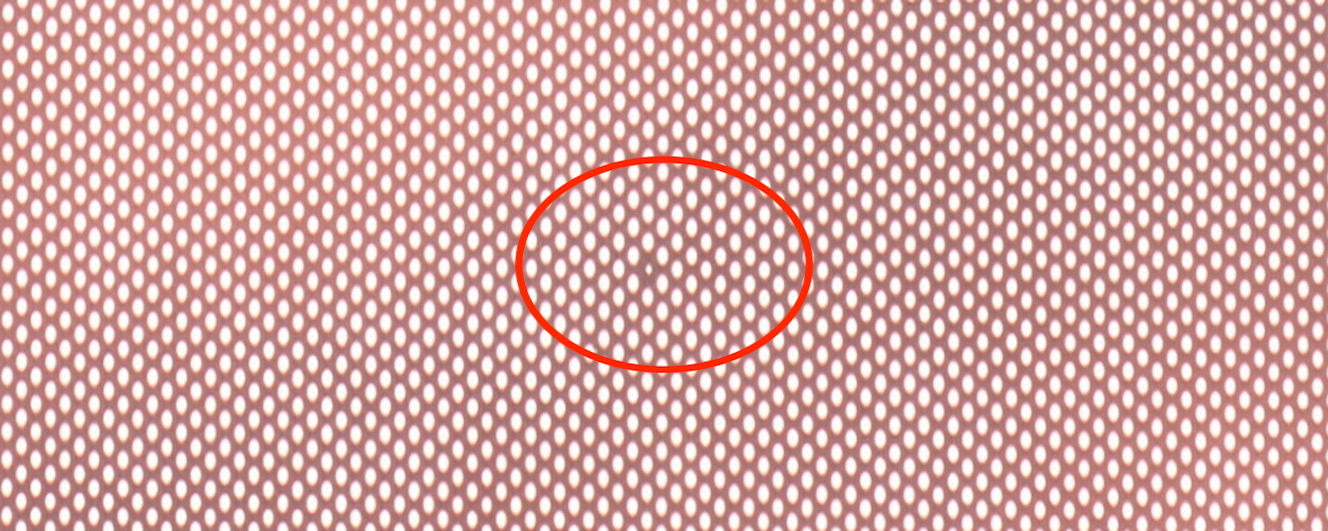
\includegraphics[width=4cm, height=3cm]{figures/GEM/figures/3b.jpg}
        \caption{ }
        \label{fig:O_4b}
    \end{subfigure}
    \centering
    \begin{subfigure}[b]{0.29\textwidth}
        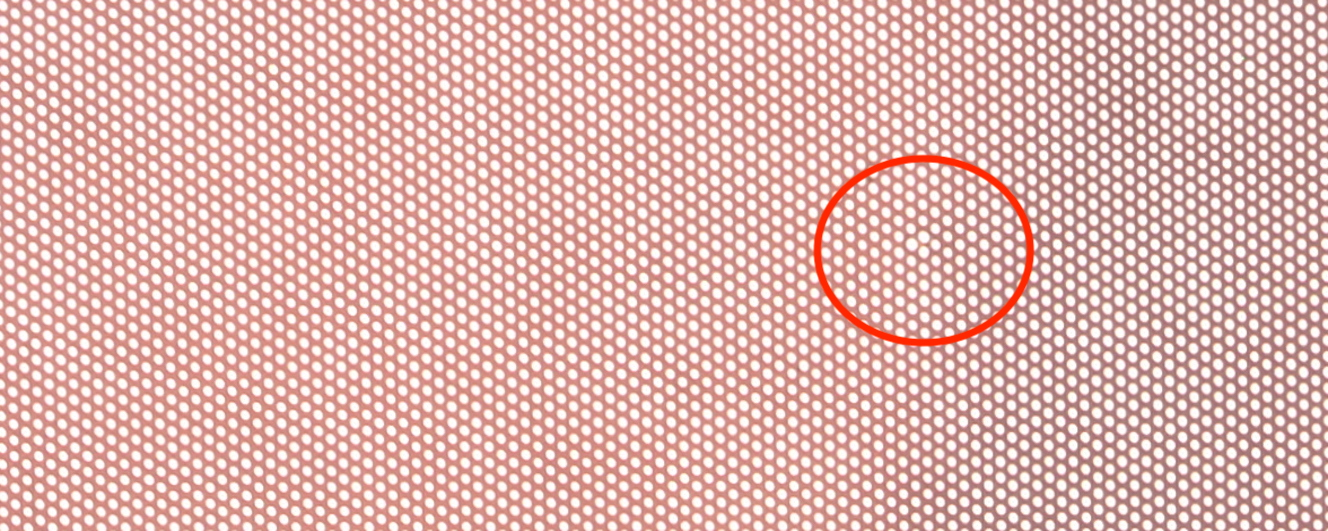
\includegraphics[width=4cm, height=3cm]{figures/GEM/figures/3c.jpg}
        \caption{ }
        \label{fig:O_4c}
    \end{subfigure}
    \centering
    \begin{subfigure}[b]{0.29\textwidth}
        \includegraphics[width=4cm, height=3cm]{figures/GEM/figures/3d.jpg}
        \caption{ }
        \label{fig:O_5a}
    \end{subfigure}
    \centering
    \begin{subfigure}[b]{0.29\textwidth}
        \includegraphics[width=4cm, height=3cm]{figures/GEM/figures/3e.jpg}
        \caption{ }
        \label{fig:O_5b}
    \end{subfigure}
    \centering
    \begin{subfigure}[b]{0.29\textwidth}
        \includegraphics[width=4cm, height=3cm]{figures/GEM/figures/3f.jpg}
        \caption{ }
        \label{fig:O_5c}
    \end{subfigure}
   \caption{Observed imperfections in the GEM foils: (a) Un-etched area, (b) under-size hole, (c) over-size hole (d) missing hole, (e) excess etching and (f) burnt area.} \label{fig:Optical_01}
\end{figure}
\begin{figure}[!htbp]
    \centering
    \begin{subfigure}[b]{0.49\textwidth}
        \includegraphics[width=7.6cm, height=5.5cm]{figures/GEM/figures/Apical_Defects.pdf}\qquad
        \caption{ }
        \label{fig:O_9a}
    \end{subfigure}
    \begin{subfigure}[b]{0.49\textwidth}
        \includegraphics[width=7.6cm, height=5.5cm]{figures/GEM/figures/CopperDefects.pdf}
        \caption{ }
        \label{fig:O_9b}
    \end{subfigure}
   \caption{Number of defects seen in (a) Insulator (Apical Type NP) and (b) Copper, for one of the 10 cm $\times$ 10 cm foil.} \label{fig:Optical_04}
\end{figure}
% subsection optical_test (end)

\subsection{Electrical Test} % (fold)
\label{sub:electrical_test}
This is one of the most important test for the GEM foil, which deals with the measurement of leakage or dark current.
Dark current exceeding the prescribed limits could lead to a short circuit in the foil thereby damaging the foil permanently.
A spark can also be produced due to presence of dust particle on the GEM foil, hence, the cleanliness of GEM foils is also ensured during this test.
% This is one of the most important tests which can tell us about the short circuit of the two copper foil, using the leakage current measurement.
% Also, it helps us to clean the GEM foil for few dust that can be seen/hear as a spark.
But, if there are the huge number of frequent spark happens then we should quickly stop the electricity and clean the foil properly.
The electricity test are carried out for foils in two steps as per the CERN standards~\cite{Abbaneo2015}:
% In order to qualify the foils the electrical test is divided into two steps as per the CERN standard~\cite{Abbaneo2015}:
\begin{enumerate}
    \item Quality control fast or QC-fast and
    \item Quality control for long or QC-long.
\end{enumerate}
QC-long and QC-short test differ in terms of the duration for which high voltage is applied to the detector to monitor its leakage current.
% The difference between QC-fast and QC-long lies in the applying voltage for shorter or longer period of time respectively and monitor the current.
Other difference is that QC-fast gives us a quick result about the leakage current or electrical connectivity of the foils while QC long provides the behaviour of foil at high voltages and gives us the actual leakage current and the number of discharges if present.
\subsubsection{QC-fast} % (fold)
\label{ssub:qc_fast}
This test is performed using the insulation tester MIT Megger 420~\cite{twelve}. This test confirms that the foil have good electrical connectivity. As the 550 V potential is applied across the GEM foil for about a minute and current did not exceed 10 $nA$ and the resistivity in the air between the two foil exceeds 2 $G\Omega$.
% \begin{figure}[!htbp]
%     \centering
%     \includegraphics[width=0.45\textwidth]{figures/GEM/megger.png}
%     \caption{caption}
%     \label{fig:label}
% \end{figure}
% subsubsection qc_fast (end)

\subsubsection{QC-long} % (fold)
\label{ssub:qc_long}
For this, the measurement the electronics set-up is shown in Fig.~\ref{fig:Cleaning_Measurement}. It consists of a GEM foil enclosed in a Plexiglass enclosure in which nitrogen gas is continuously floated. The foil is connected to a the Keithley 6517B picoammeter~\cite{Keithley-6517B-picoammeter} interfaced with a computer via a GPIB interface and the LabView program is used to record the measurements. The leakage current is measured as a function of applied voltage as shown in Fig.~\ref{fig:Indian_foils_H20}. Also, for the sake of comparison same measurement was made with $10~cm~\times~10~cm$ GEM foil produced at CERN. The results using the CERN foil is shown in Fig.~\ref{fig:CERN_foils}. It is observed that the two foils, one produced by Micropack and another produced at CERN, show similar behaviour and the leakage currents are well within the limit (10 $nA$), set by CERN QC criteria.
% subsubsection qc_long (end)
\begin{figure}[!htbp]
    \centering
    %\begin{subfigure}[b]{0.7\textwidth}
        \includegraphics[width=12cm,height=8cm]{figures/GEM/figures/10.jpeg}
        %\includegraphics[width=12.0cm, height=9.0cm]{figures/GEM/figures/Electrical_Sketch.png}
    %    \caption{ }
        %\label{fig:Setup}
    %\end{subfigure}
   \caption{Sketch of the set-up used for the measurement of leakage current.} \label{fig:Cleaning_Measurement}
\end{figure}
%=====================================================================
\begin{figure}[!htbp]
    \centering
    \begin{subfigure}[b]{0.5\textwidth}
        %\includegraphics[width=7.5cm, height=5.5cm]{Indian_foils_H20.pdf}
        \includegraphics[width=7.5cm, height=5.5cm]{figures/GEM/figures/Fig_11(a).pdf}
        \caption{ }
        \label{fig:Indian_foils_H20}
    \end{subfigure}
    \begin{subfigure}[b]{0.46\textwidth}
        %\includegraphics[width=7.5cm, height=5.5cm]{CERN_foils.pdf} 
        \includegraphics[width=7.5cm, height=5.5cm]{figures/GEM/figures/Fig_11(b).pdf} 
        \caption{ }
        \label{fig:CERN_foils}
    \end{subfigure}
   \caption{Leakage Current for (a) Micropack Foils and (b) CERN Foils, at an average temperature of T=27$^{\circ}$ C and 20\% relative humidity.} \label{fig:L_01}
\end{figure}

% subsection electrical_test (end)
% section characterization_and_production_of_gem_foil (end)

% \section{Summary} % (fold)
% \label{sec:summary}
% First time the GEM foils are produced in India using TOT agreement between CERN and Micropack Pvt. Ltd. Micropack 

% Efficiency and time resolution are important parameters for a gaseous detectors. Efficiency is defined as the ratio of events reconstructed by tracker+GEM to the number of events reconstructed by tracker only. Experimentally, the time resolution is calculated using the root mean square of the Gaussian distribution of the time taken by a particle to reach the detector from the scintillator. Further, we applied a fast 40MHz clock pulse to cope up with the LHC bunch crossing. Thus, the detector's time response should be modelled as the Gaussian function convoluted with a square wave function having frequency 40MHz. To achieve the time resolution we fit the experimental data with the Gaussian function convoluted with the square wave and then using fit parameters we extracted the time resolution before convolution. Finally, we obtained the very good time resolution of ~7ns and efficiency ~98\% with both gas mixture Ar/CO$_2$ (70/30) and Ar/CO$_2$/CF$_4$ (45/15/40), as shown in Fig. \ref{Efficiency} and \ref{TimeResolution}.  At the end, by comparing the results of two different gas mixture  we can  conclude that GEM detectors can be operated without using CF$_4$, while maintaining its performance.


% GEM foils were produced for the first time in India under the TOT agreement between Micropack Pvt. Ltd. and CERN. Micropack started the preparations for the GEM foil production in India. The first few attempts saw many deviations from the required quality. With further improvements in etching technology and several rounds of iterations, Micropack finally produced a batch of foils which appeared fine from visual inspection and preliminary checks. However, before these foils could be declared fit for applications and technology as reliable, we had to perform the desired quality assessment and characterization for these foils. For this purpose, we performed optical and electrical tests to check the reliability and usability of the foils. Optical tests reveal that the holes are quite uniform with inner and outer diameters of 49.9 $\pm$ 1.6 $\mu$m and 70.01 $\pm$ 2.02 $\mu$m respectively. Here, the quoted errors are the Gaussian one sigma uncertainty on diameter distributions. A current of less than 1 nA has been observed in dry nitrogen environment from electrical measurements and were in agreement with CERN foils. The measured optical and electrical properties of Micropack foils were found to reflect the desired parameters and are at par with the double mask foils produced at CERN. With the successful production of 10 cm $\times$ 10 cm double-mask GEM foils, Micropack has already extended their infrastructure to handle single-mask technology so that larger foils can be produced in order to ease the commercialization of large area GEM foils.

% section summary (end)